\chapter{Mutant npat results in nucleosome positioning defects in \textit{D. rerio} CMZ progenitors, blocking specification but not proliferation}
\chaptermark{Nucleosome position and specification defects in npat mutant \textit{rys}}
\label{chap:rys}
\section{Introduction}
The zebrafish (D. rerio) circumferential marginal zone (CMZ), located in the retinal periphery, contains the retinal stem cells and progenitors responsible for the lifelong retinal neurogenesis observed in this cyprinid. Analagous to CMZs in other model organisms, such as X. laevis \cite{Perron1998}, it has been of particular interest to us since the discovery of quiescent stem cells at the mammalian retinal periphery \cite{Tropepe2000}, as an understanding of the molecular mechanisms regulating this proliferative zone may shed light on whether these mammalian cells might be harnessed for the purpose of regenerative retinal medicine. While significant progress has been made in this direction \cite{Raymond2006}, molecular lesions in a plethora of zebrafish mutants displaying defects in CMZ development and activity remain largely uncharacterised. We examine here one such micropthalmic line identified in an ENU screen, \textit{rys} \cite{Wehman2005}, characterised by Wehman et al. as a Class IIA CMZ mutant, with a small eyes (see \autoref{ryspic}) and apparently paradoxically enlarged CMZ.

\begin{figure}[!h]
    \makebox[\textwidth][c]{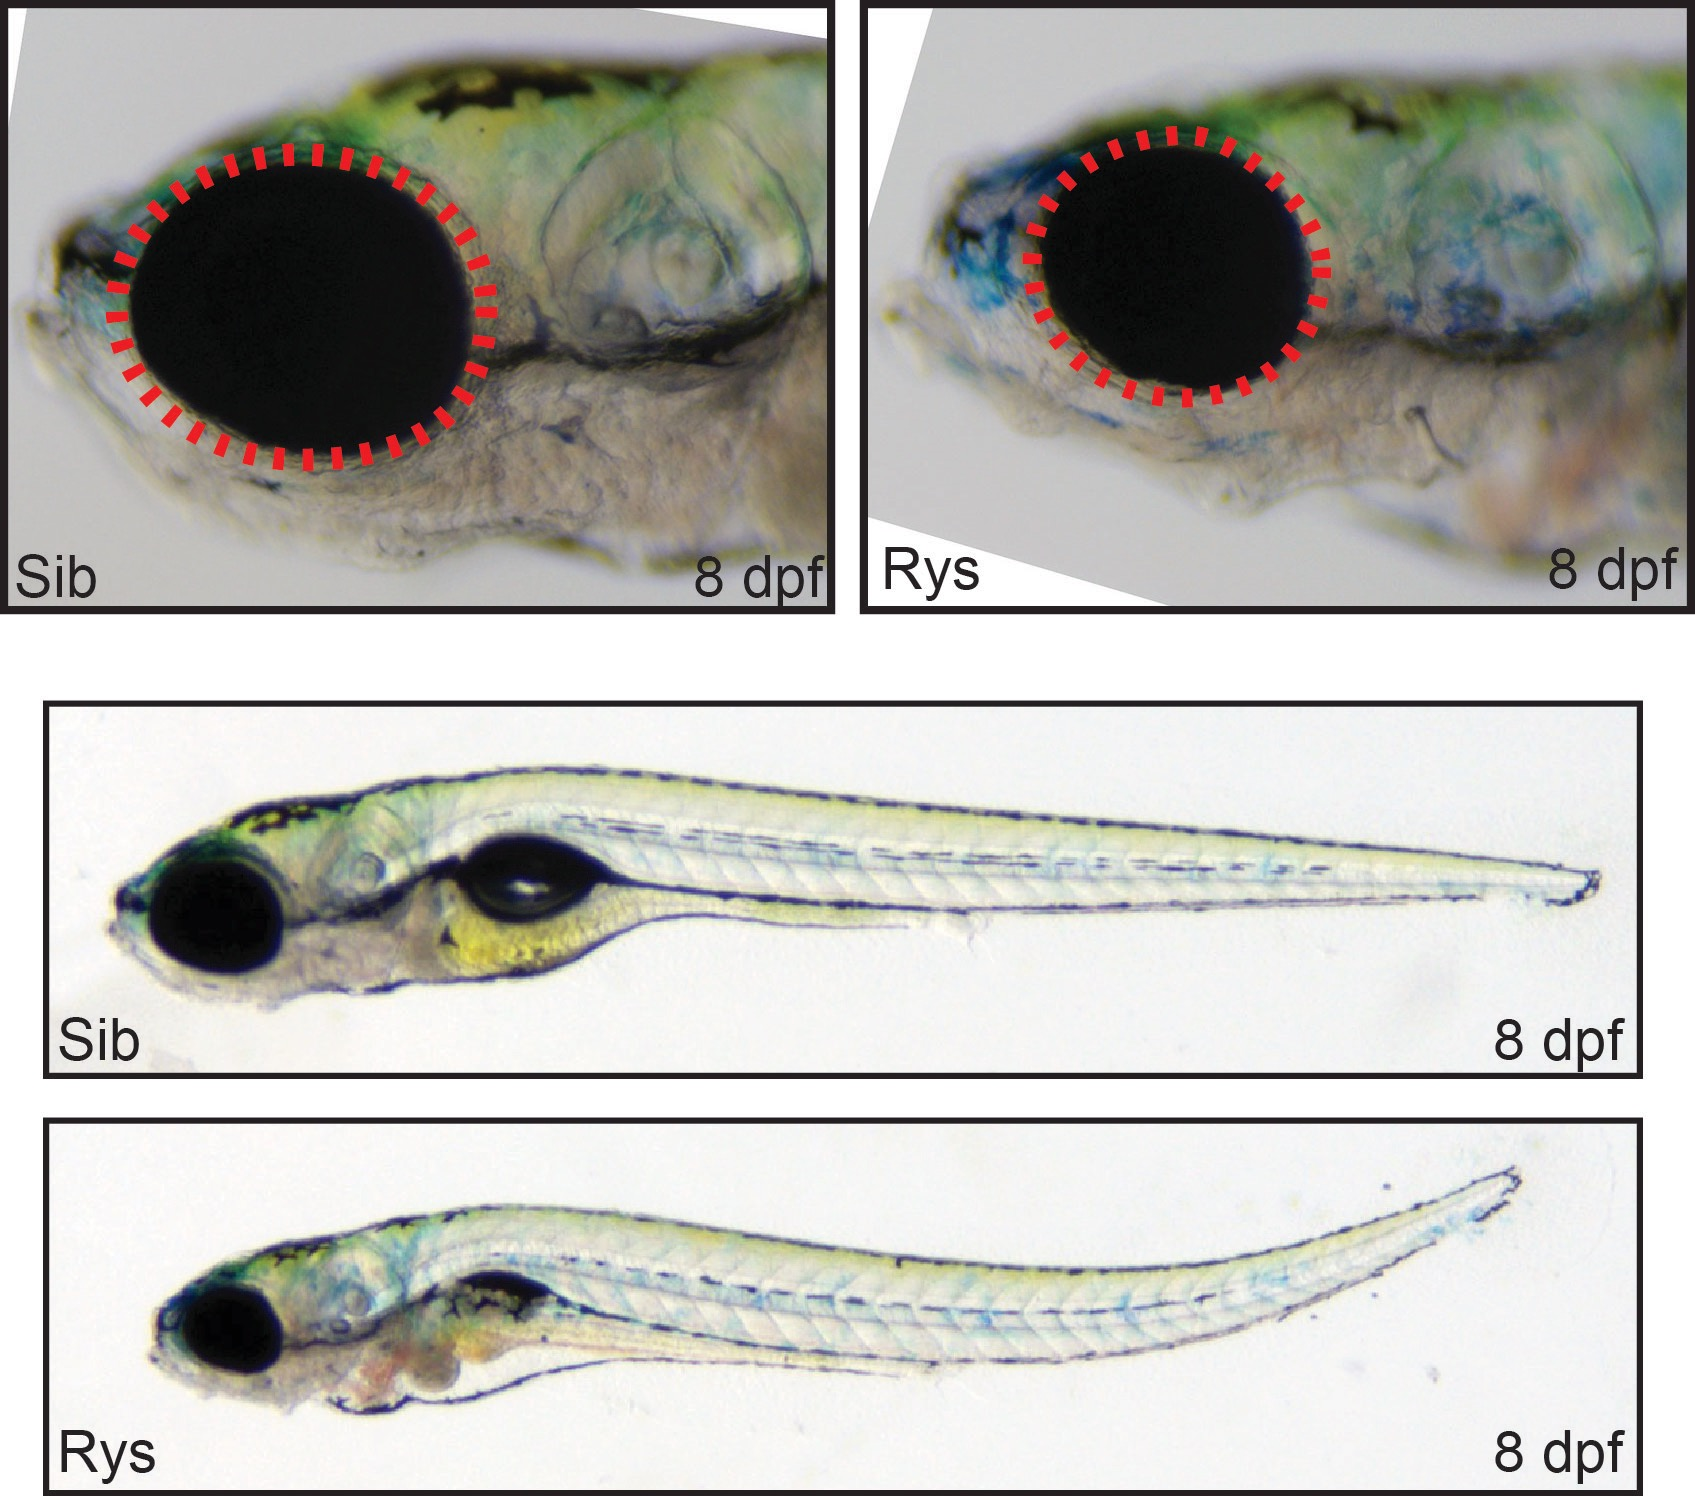
\includegraphics[width=.6\textwidth]{rys/rys.jpg}}    
    \caption{{\bf \textit{rys} mutants exhibit a small-eye phenotype}}
    \label{ryspic}
    8 dpf \textit{rys} sibling (Sib) and mutant (Rys), head area (top panels), whole body (bottom panels). Red dashes highlight the overall reduced eye size in homozygous \textit{rys} mutant animals.
\end{figure}

Mapping revealed the causative \textit{rys} mutation lay in the zebrafish npat gene, the nuclear protein associated with the ataxia-telangiectasia locus in mammals \cite{Imai1996}. Although npat is heretofore uncharacterised in zebrafish, its mammalian homologues, human NPAT and mouse Npat, have been extensively examined. These studies have demonstrated that NPAT plays a critical role in coordinating events associated with the G1/S phase transition in proliferating cells \cite{Ye2003}. S-phase entry requires tight co-ordination between the onset of genomic DNA synthesis and histone production, in order to achieve normal chromatin packaging and assembly. NPAT, found in the nucleus \cite{Sagara2002} and localised, in a cell-cycle dependent manner, to histone locus bodies \cite{Ghule2009}, induces S-phase entry \cite{Zhao1998} and activates replication-dependent histone gene transcription by direct interaction with histone gene clusters \cite{Zhao2000} in association with histone nuclear factor P (HiNF-P) \cite{Mitra2003}. The protein’s effects on S-phase entry and histone transcription are associated with distinct domains at the C-terminus and N-terminus, respectively \cite{Wei2003}. NPAT is also known to associate with the histone acetyltransferase CBP/p300 \cite{Wang2004} and directs histone acetylation by this enzyme \cite{He2011}.

NPAT is known to be a component of the E2F transcriptional program \cite{Gao2003} and a substrate of cyclin E/CDK2 \cite{Zhao1998}, although E2F-independent activation by cyclin D2/CDK4 in human ES cells has also been described \cite{Becker2010}. The expression of NPAT protein peaks at the G1/S boundary \cite{Zhao1998}, as does its phosphorylation, which promotes its transcriptional activation of replication-dependent H2B \cite{Ma2000} and H4 \cite{Mitra2009} genes, while its effect on low, basal levels of H4 transcription is phosphorylation-independent \cite{Ye2003}. Of particular interest, NPAT has recently been found to be required for CDK9 recruitment to replication-dependent histone genes \cite{Pirngruber2010}; CDK9 and monoubiquitinated H2B are essential for proper 3’ end processing of stem-loop histone transcripts \cite{Pirngruber2009}. NPAT and HiNF-P have also been found associated with the U7 snRNP complexes that perform this function \cite{Ghule2009}. The replication-dependent activities of NPAT are thought to be terminated by WEE1 phosphorylation of H2B, which excludes NPAT from histone clusters \cite{Mahajan2012}.

All of these studies have been conducted in tissue culture contexts, perhaps due to the challenges associated with studying this critical protein in vivo; mouse embryos with provirally inactivated Npat arrest at the 8-cell stage, for instance \cite{DiFruscio1997}. The availability of \textit{rys}, a zebrafish npat mutant which develops well into the larval stage, is therefore of considerable interest, as it allows for the study of npat’s function within complete tissues. We demonstrate here that npat is critical for the normal proliferation and differentiation of CMZ neural progenitors.

We find substantial evidence for the role of \textit{D. rerio} npat involvement with histone transcription, nucleosome positioning, and scheduling of mitotic activity; we suggest that the \textit{rys} phenotype is brought about by a failure to coordinate the genomic states required to specify, independently of proliferative capacity, in postembryonic zebrafish RPCs of the CMZ.

\section{Results}
\subsection{The \textit{rys} CMZ phenotype is characterised failure of RPCs to specify, altered nuclear morphology, aberrant proliferation and expanded early progenitor identity}

\textit{rys} has previously been described as having an enlarged CMZ \cite{Wehman2005}, but whether this is a consequence of an enlarged proliferative population, altered cellular morphology, or other causes, remained unclear. We sought to learn more about the ontogeny of the mutant niche by examining two histochemical markers of cycle activity during the early life of \textit{rys}; Proliferating Cell Nuclear Antigen (PCNA), which in \textit{D. rerio} is expressed throughout the cell cycle, and the genomic incorporation of the thymidine analogue EdU over a 24 hour pulse, which indelibly marks cells that have passed through S-phase whilst exposed to it. These data are displayed in \autoref{rysCMZontogeny}. During this period, the PCNA positive population of the sibling CMZ declines precipitously (Panel A), with a corresponding decrease in proliferative activity as measured by the incorporation of EdU (Panel B). Whether or not the \textit{rys} CMZ population is enlarged by comparison depends on the age at which it is sampled, with there is a 99.6\% probability of the posterior mean sectional \textit{rys} CMZ PCNA population being below the sib mean at 4dpf, while 99.8\% of the marginal posterior of the 10dpf \textit{rys} mean lies above that of sibs. Therefore, the \textit{rys} CMZ population is better described as achieving its peak periembryonic size later than siblings; its population is only numerically larger than sibs at later ages\footnote{\textit{rys} animals universally die by approximately 3 weeks of age.}. 

\begin{figure}[!h]
    \makebox[\textwidth][c]{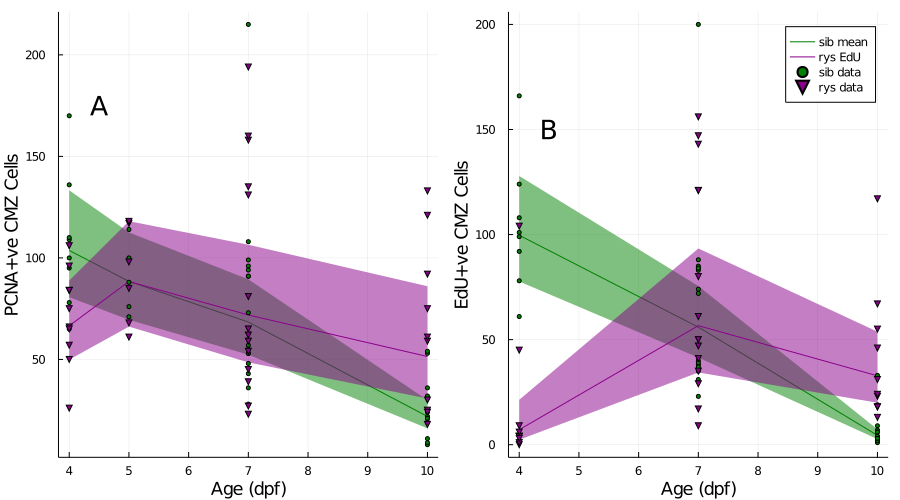
\includegraphics[width=1.\textwidth]{rys/CMZontogeny.png}}    
    \caption{{\bf \textit{rys} CMZ populations start relatively small and quiescent, end abberantly large and proliferative}}
    Panel A: Counts and estimated mean $\pm$95\% credible intervals of PCNA-positive cells in the peripheral CMZ of \textit{rys} (magenta) and their siblings (green)
    Panel B: As above, but for counts of double PCNA-,EdU-positive cells in the CMZ after a 24 hour pulse of EdU.
    \label{rysCMZontogeny}

\end{figure}
\FloatBarrier

Surprisingly, very few \textit{rys} animals have many actively cycling RPCs at 4dpf, by comparison to the robustly cycling sib RPCs at this age; a mean estimate of 96.2$\pm$3.4\% of sib RPCs are labelled during the 24 hr pulse at 4dpf, while only 24.1$\pm$37.2\% of \textit{rys} RPCs are. The situation is broadly reversed at 10dpf, with only 24.4$\pm$14.9\% of sib RPCs labelled, compared to 65.8$\pm$16.2\% of \textit{rys} RPCs. While we questioned whether this late-stage increase in \textit{rys} thymidine analogue labelling might not represent bona fide mitotic activity, we were able to readily find mitotic figures within these populations, shown in Supplementary \autoref{rysmitosis}. As the data convey, these outcomes are highly variable in both sib and \textit{rys} animals, with, for instance, an isolated mutant at 4dpf sporting an EdU-positive population near the sibling mean. However, even in those \textit{rys} animals which do have actively proliferating RPCs at these earlier ages, there is a marked failure of the CMZ to contribute to the postmitotic, specified neural retina. Confocal micrographs displaying \textit{rys} CMZ cohorts labelled with BrdU at 3dpf that have failed to enter the neural retina after 7 days of chase time are displayed alongside their normal siblings in \autoref{contributionfailure}. 

\begin{figure}[!h]
    \makebox[\textwidth][c]{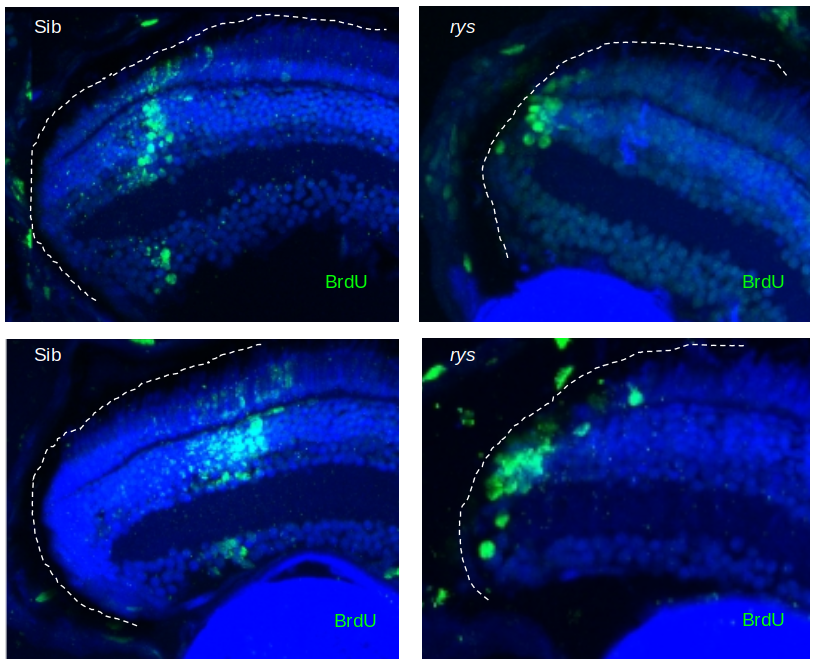
\includegraphics[width=1.\textwidth]{rys/cmzfailure.png}}    
    \caption{{\bf \textit{rys} CMZ RPCs fail to contribute to the neural retina}} M
    14\si{\micro\metre} coronal cryosections through representative sib (left panels) and \textit{rys} eyes at 10dpf, 7 days after an 8hr BrdU pulse at 3dpf. Note that few labelled \textit{rys} cells have entered the specified retinal layers.
    \label{contributionfailure}
\end{figure}
\FloatBarrier

Indeed, a close study of the 5dpf retinae, held back from EdU processing to preserve their nuclear features (presented in \autoref{nuclearstudy}), suggests that the primary reason for the enlarged appearance of \textit{rys} CMZs, even at this age, when the niche's population is numerically similar to siblings (Panel A), is this failure to contribute to the neural retina, leading to \textit{rys} central retinae that are about half as populous, per cell of the CMZ, as their siblings (Panel B). This appearance may be enhanced in the dorsal CMZ, there is an  87.8\% probability that the posterior mean for this region in \textit{rys} is above the sibling mean, although this is compensated for by 97.5\% of the marginal posterior distribution on the ventral mean laying below the same sibling mean (Panels C and D). More significantly, \textit{rys} nuclei tend to be much larger than their siblings (Panel E), as well as consistently less spherical (Panel F).

\begin{figure}[!h]
    \makebox[\textwidth][c]{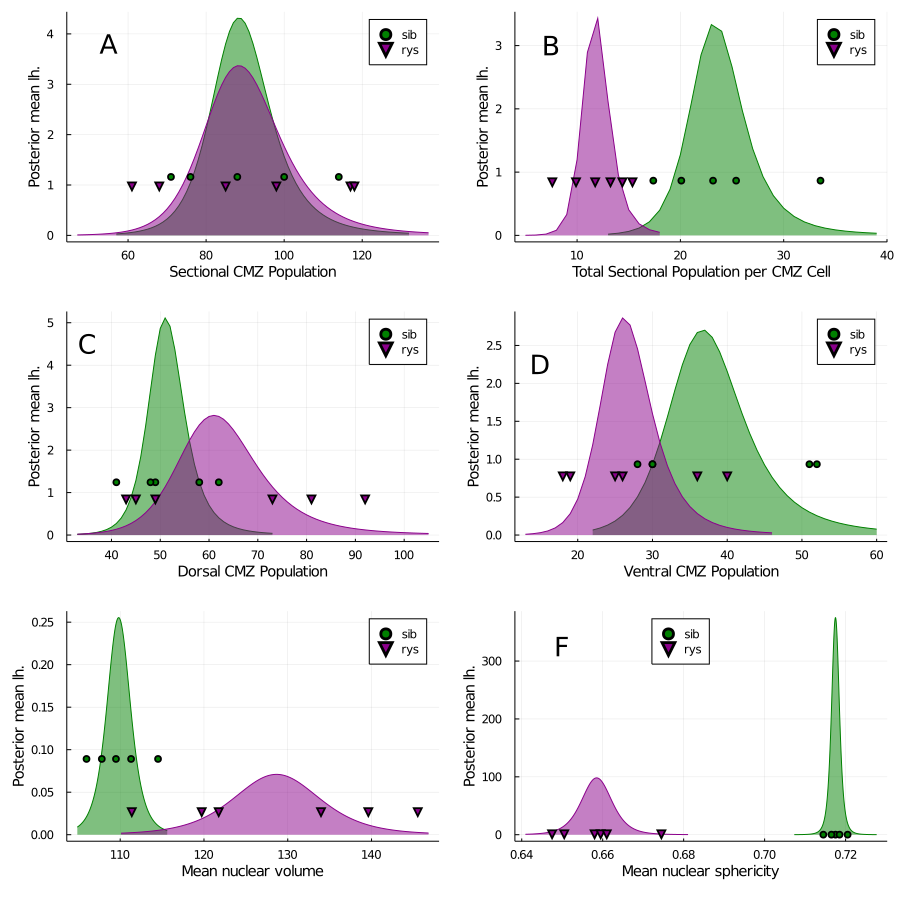
\includegraphics[width=1.\textwidth]{rys/nuclearstudy.png}}    
    \caption{{\bf 7dpf \textit{rys} CMZ RPCs display enhanced asymmetry, increased volume, decreased sphericity, and relative but not absolute enlargement}}
    \label{nuclearstudy}
    All panels display sib observations as green circles and \textit{rys} as magenta triangles. Plotted behind the underlying observations are the calculated marginal posterior distributions of the mean, given log-Normal models of the population data and Normal models of the volume and sphericity data. The y-axis shows the relative likelihood of underlying mean values on the x-axis, given the data.
    Panel A: Total dorsal + ventral CMZ population per central coronal section.
    Panel B: Number of PCNA negative, specified central retinal neurons per PCNA postive CMZ cell.
    Panels C and D: Dorsal and Ventral CMZ populations per central coronal cryosection.
    Panel E: Mean volume of nuclei in a given individual's central coronal cryosection.
    Panel F: Mean sphericity of nuclei in a given individual's central coronal cryosection.
\end{figure}

In order to quantitiatively rank these contributions to the \textit{rys} nuclear phenotype, we calculated the evidence for combined LogNormal (population measurements) and Normal (nuclear measurements) models of sib and rys data, against the joint evidence for separate models. These estimates are presented in \autoref{nuclearev}. Our measurements indicate that the best evidentiated contributors to the \textit{rys} CMZ phenotype are, first, the decrease of nuclear sphericity, followed by the decreased number of central retinal neurons relative to the CMZ, then, the increase in nuclear volume, and lastly the expansion of the dorsal CMZ. These calculations also demonstrate that there is no evidence for overall differences in sectional CMZ population, and that the ventral CMZ is less populous in \textit{rys}, which may contribute to the appearance of an enlarged dorsal CMZ. The large size of the nuclear morphological changes and the decreased number of central cells indicates that these are the most important contributors to the \textit{rys} phenotype.

\begin{table}[!ht]
    \centering
    \caption{{\bf Evidence-based ranking of phenomenal contributors to \textit{rys} phenotype}}
    \begin{tabular}{|l|l|l|l|l|} 
        \hline {\bf Parameter} & {\bf Separate logZ} & {\bf Combined logZ} & {\bf logZR} & {\bf $\sigma$ sign.}\\ \hline 
        Sectional CMZ pop. & -280.8 ± 1.7 & {\bf -183.44 ± 0.9} & -97.4 ± 1.9 & 50.7 \\ \hline
        Central pop./CMZ cell & {\bf -62.51 ± 0.64} & -89.88 ± 0.12 & 27.38 ± 0.66 & 41.7 \\ \hline
        Dorsal CMZ pop.  & {\bf -180.1 ± 1.0} & -192.8 ± 1.1 & 12.8 ± 1.5 & 8.3 \\ \hline
        Ventral CMZ pop. & {\bf -136.86 ± 0.32} & -147.36 ± 0.46 & 10.5 ± 0.56 & 18.8 \\ \hline
        Nuclear Volume & {\bf -164.18 ± 0.29} & -229.3 ± 1.9 & 65.1 ± 1.9 & 34.4 \\ \hline
        Nuclear Sphericity & {\bf -89.1 ± 1.8} & -311.2 ± 3.9 & 222.0 ± 4.2 & 52.3 \\ \hline
    \end{tabular}
    \label{nuclearev}
\end{table}


\FloatBarrier

\begin{figure}[!h]
    \makebox[\textwidth][c]{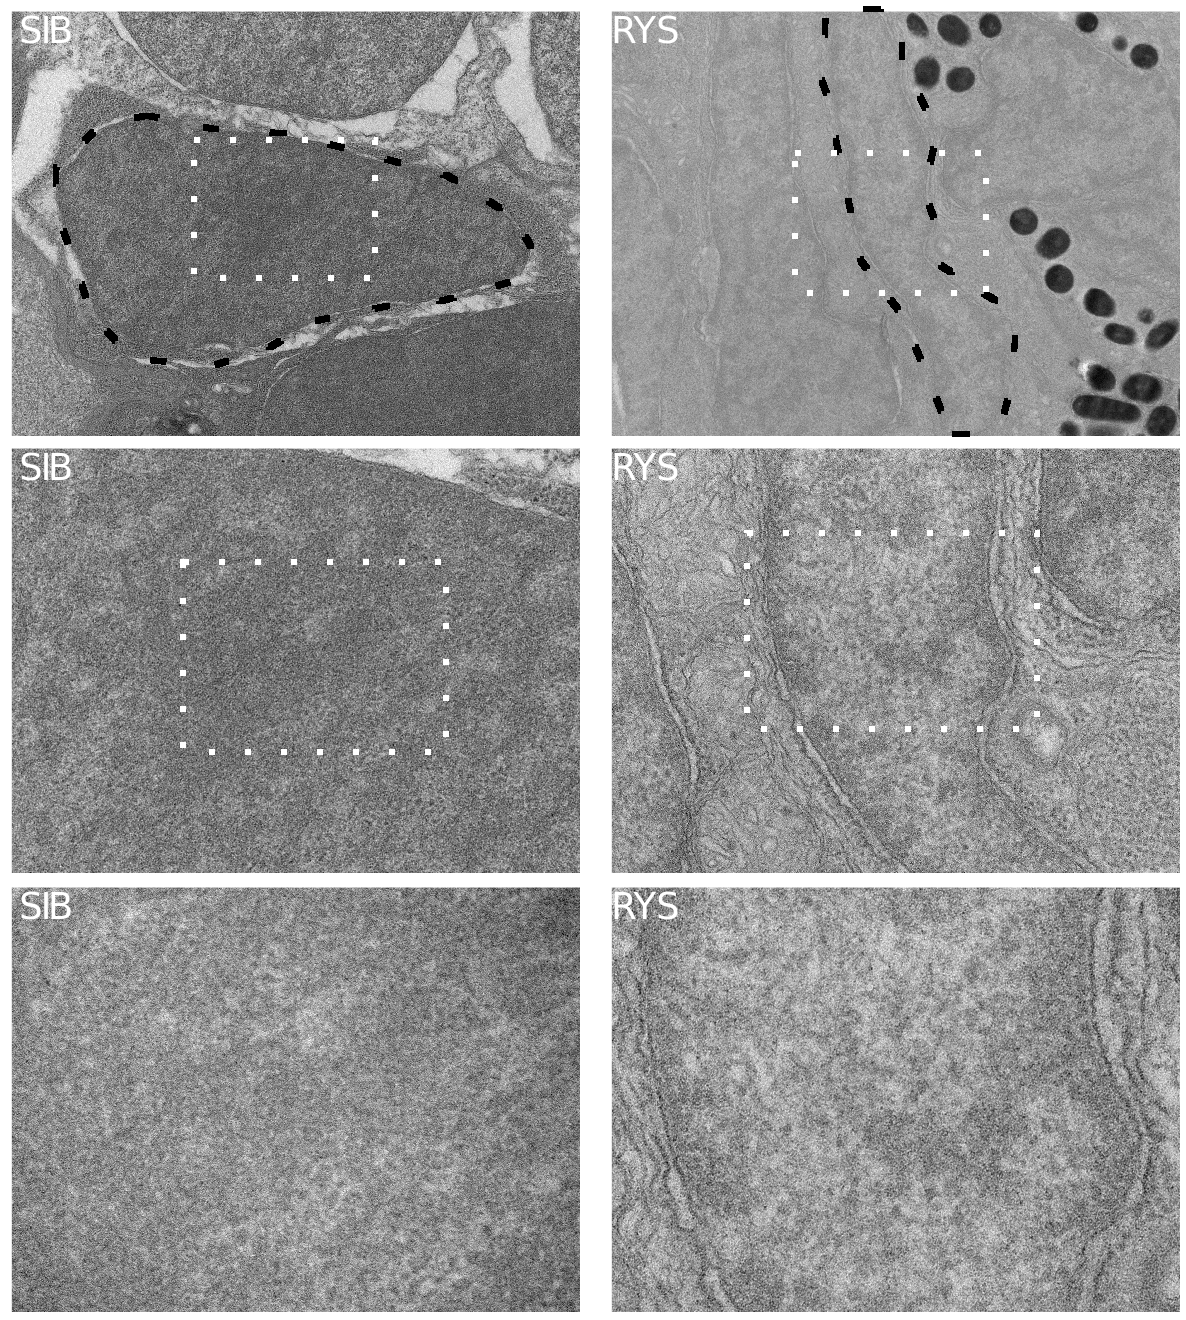
\includegraphics[width=.8\textwidth]{rys/rysem.png}}    
    \caption{{\bf RPC nuclei of the \textit{rys} CMZ display disorganized, loosely packed chromatin}}
    Representative electron micrographs of \textit{rys} sibling and mutant CMZ RPC nuclei.
    Left panels: siblings. Right panels: \textit{rys}. Top panels: 36000x magnification, general overview of the area around the nucleus, dashed black. Area displayed in middle panels dashed white. Middle panels: 110000x magnification nuclear detail. Area displayed in bottom panels dashed white. Bottom panels: 210000x magnification, chromosomal ultrastructure.
    \label{rysEM}
\end{figure}

The characteristically enlarged nuclei in \textit{rys} have a billowy appearance suggestive of chromosomal disorganization. In order to investigate this possibility further, we used electron microscopy to examine the nuclear ultrastructure of RPC nuclei in \textit{rys} and sibling CMZs. Representative electron micrographs are presented in \autoref{rysEM}. At 36000x magnification, the unusual and disorganized structure of \textit{rys} nuclei become apparent, particularly in contrast with the consistently teardrop-shaped nuclei of sibling RPCs; the \textit{rys} nucleus pictured is so pancaked it extends out of the frame that readily captures a sibling nucleus. When the chromatin itself is imaged at 210000x magnification, it appears much less electron-dense in the rys, with much larger tracts of presumptive euchromatin, and less regular spacing of chromosomal material.
\FloatBarrier

If RPCs in \textit{rys} CMZs are failing to enter the specified neural retina, but by 7dpf are becoming mitotically active, this leaves the question of why this apparently proliferative niche's population is declining by 10dpf. We suspected that \textit{rys} RPCs may be undergoing apoptosis in situ. Although we did not detect pyknotic nuclear fragments in our EM investigations, it is possible that the individual apoptotic events are too rare in \textit{rys} to reliably detect in this manner. In order to investigate this possibility, we assayed the presence of caspase-3 in \textit{rys} and sib CMZs. As displayed in \autoref{caspase}, caspase-3-positive nuclei can be detected in the \textit{rys} CMZ at both 4 and 6 dpf (mean 6.5 $\pm$ 7.5 and 2.6 $\pm$ 1.1 cells, respectively) but are not found in sib CMZs, though both display a similar level of central apoptotic activity (4dpf \textit{rys}: 1.25 $\pm$ 1.0; 4dpf sib: 1.4 $\pm$ 1.1; 6dpf \textit{rys} 0.6 $\pm$ 0.9; 6dpf sib: 1.0 $\pm$ 1.4 ). The lack of debris observable in \textit{rys} CMZs is likely attributable to the activity of 4C4-positive microglia active in the area; we observed one such cell actively phagocytosing TUNEL-labelled \textit{rys} RPC nuclear fragments in the CMZ, displayed in Supplementary \autoref{phagocytosis}.

\begin{figure}[!h]
    \makebox[\textwidth][c]{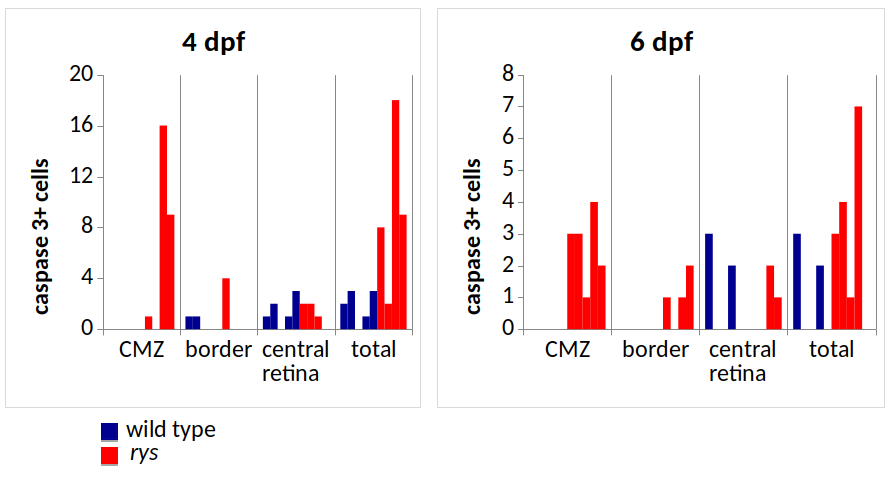
\includegraphics[width=1.\textwidth]{rys/caspase.png}}    
    \caption{{\bf \textit{rys} mutant CMZs have increased caspase-3 positive nuclei}}
    Number of caspase-3 positive cells counted in CMZ, the border between the CMZ and specified central retina, the specified central neural retina, and the overall total, at 4 dpf (left panel) and 6 dpf (right panel). One central \SI{20}{\micro\metre} section per sibling (S) and \textit{rys} (R) larva.
    \label{caspase}
\end{figure}

Suspecting that \textit{rys} CMZ RPCs may maintain an early progenitor identity, causing their failure to contribute to the specified neural retina, we examined pax6a immunostaining of this population, which is normally restricted to putative progenitors in the peripheral and middle CMZ, as well as the retinal ganglion cell layer \cite{Raymond2006}. The Pax6-stained region was enlarged in \textit{rys} CMZs relative to their siblings (\autoref{progenitoridentity}, center panels). As vsx2 is also known to be a marker of retinal progenitor cells in the CMZ \cite{Raymond2006}, we also generated a transgenic vsx2::eGFP \textit{rys} line using a fragment of the zebrafish vsx2 promoter which drives eGFP expression in the utmost retinal periphery in siblings. Mutant fish from this line displayed substantially expanded eGFP expression in the CMZ (\autoref{progenitoridentity}, right panels).

\begin{figure}[!h]
    \makebox[\textwidth][c]{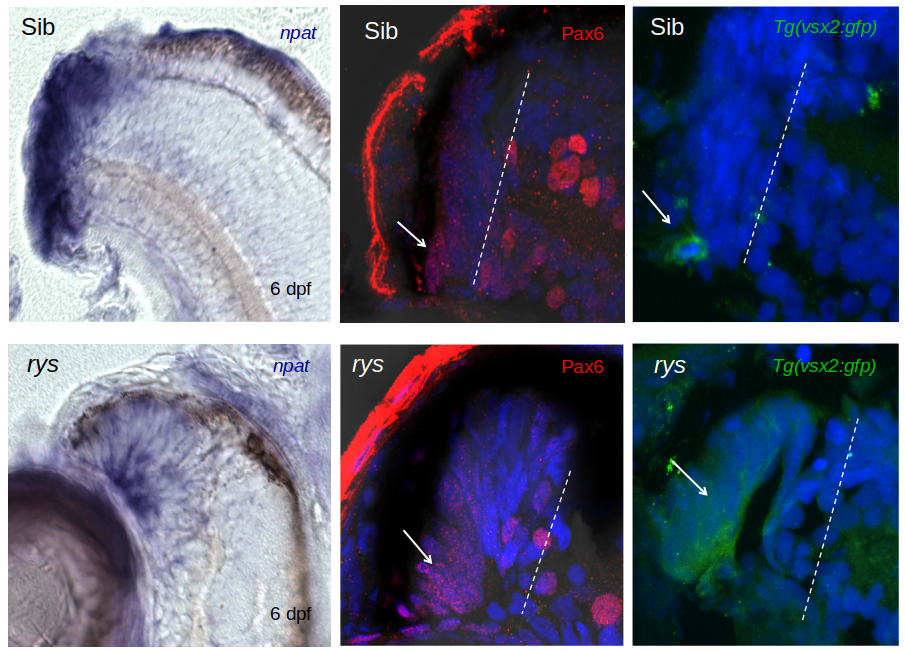
\includegraphics[width=1.2\textwidth]{rys/progenitorid.png}}    
    \caption{{\bf Mutant \textit{rys} RPCs display expanded expression of early progenitor markers}}
    Representative transmitted light and confocal micrographs of \textit{rys} sibling and mutant CMZ RPCs. Top panels: siblings. Bottom panels: \textit{rys} mutants. Left panels: in-situ hybridization using npat probe on 20\si{\micro\metre} coronal cryosection. Middle panels: anti-Pax6 immunohistochemistry. Right panels: GFP expression in a Tg(vsx2:GFP) line introgressed into \textit{rys}. 
    \label{progenitoridentity}
\end{figure}

\FloatBarrier
\subsection{The micropthalmic zebrafish line \textit{rys} is an npat mutant}

In order to determine the causative mutation responsible for the \textit{rys} phenotype, we performed linkage mapping to identify candidate genes, followed by PCR analysis of the transcript products of these candidates. This study revealed a single G\textgreater{}A transition at position 24862961 on chromosome 15 (NC\_007126.5, Zv9), annotated as the first base of intron 9 in the zebrafish npat gene, in a canonical GU splice donor site. 

We observed that this mutation reliably results in the retention of npat intron 8, and less frequently, in the retention of both introns 8 and 11, in 6dpf \textit{rys} mutants, shown in \autoref{npattranscript}. The predicted protein sequence expressed from the mutant transcript is truncated by a stop codon at residue 283, which would preclude the translation of predicted phosphorylation sites and nuclear localisation signals cognate to those identified in human NPAT \cite{Ma2000,Sagara2002}, as displayed in \autoref{npatprotein}.

\begin{figure}[!h]
    \makebox[\textwidth][c]{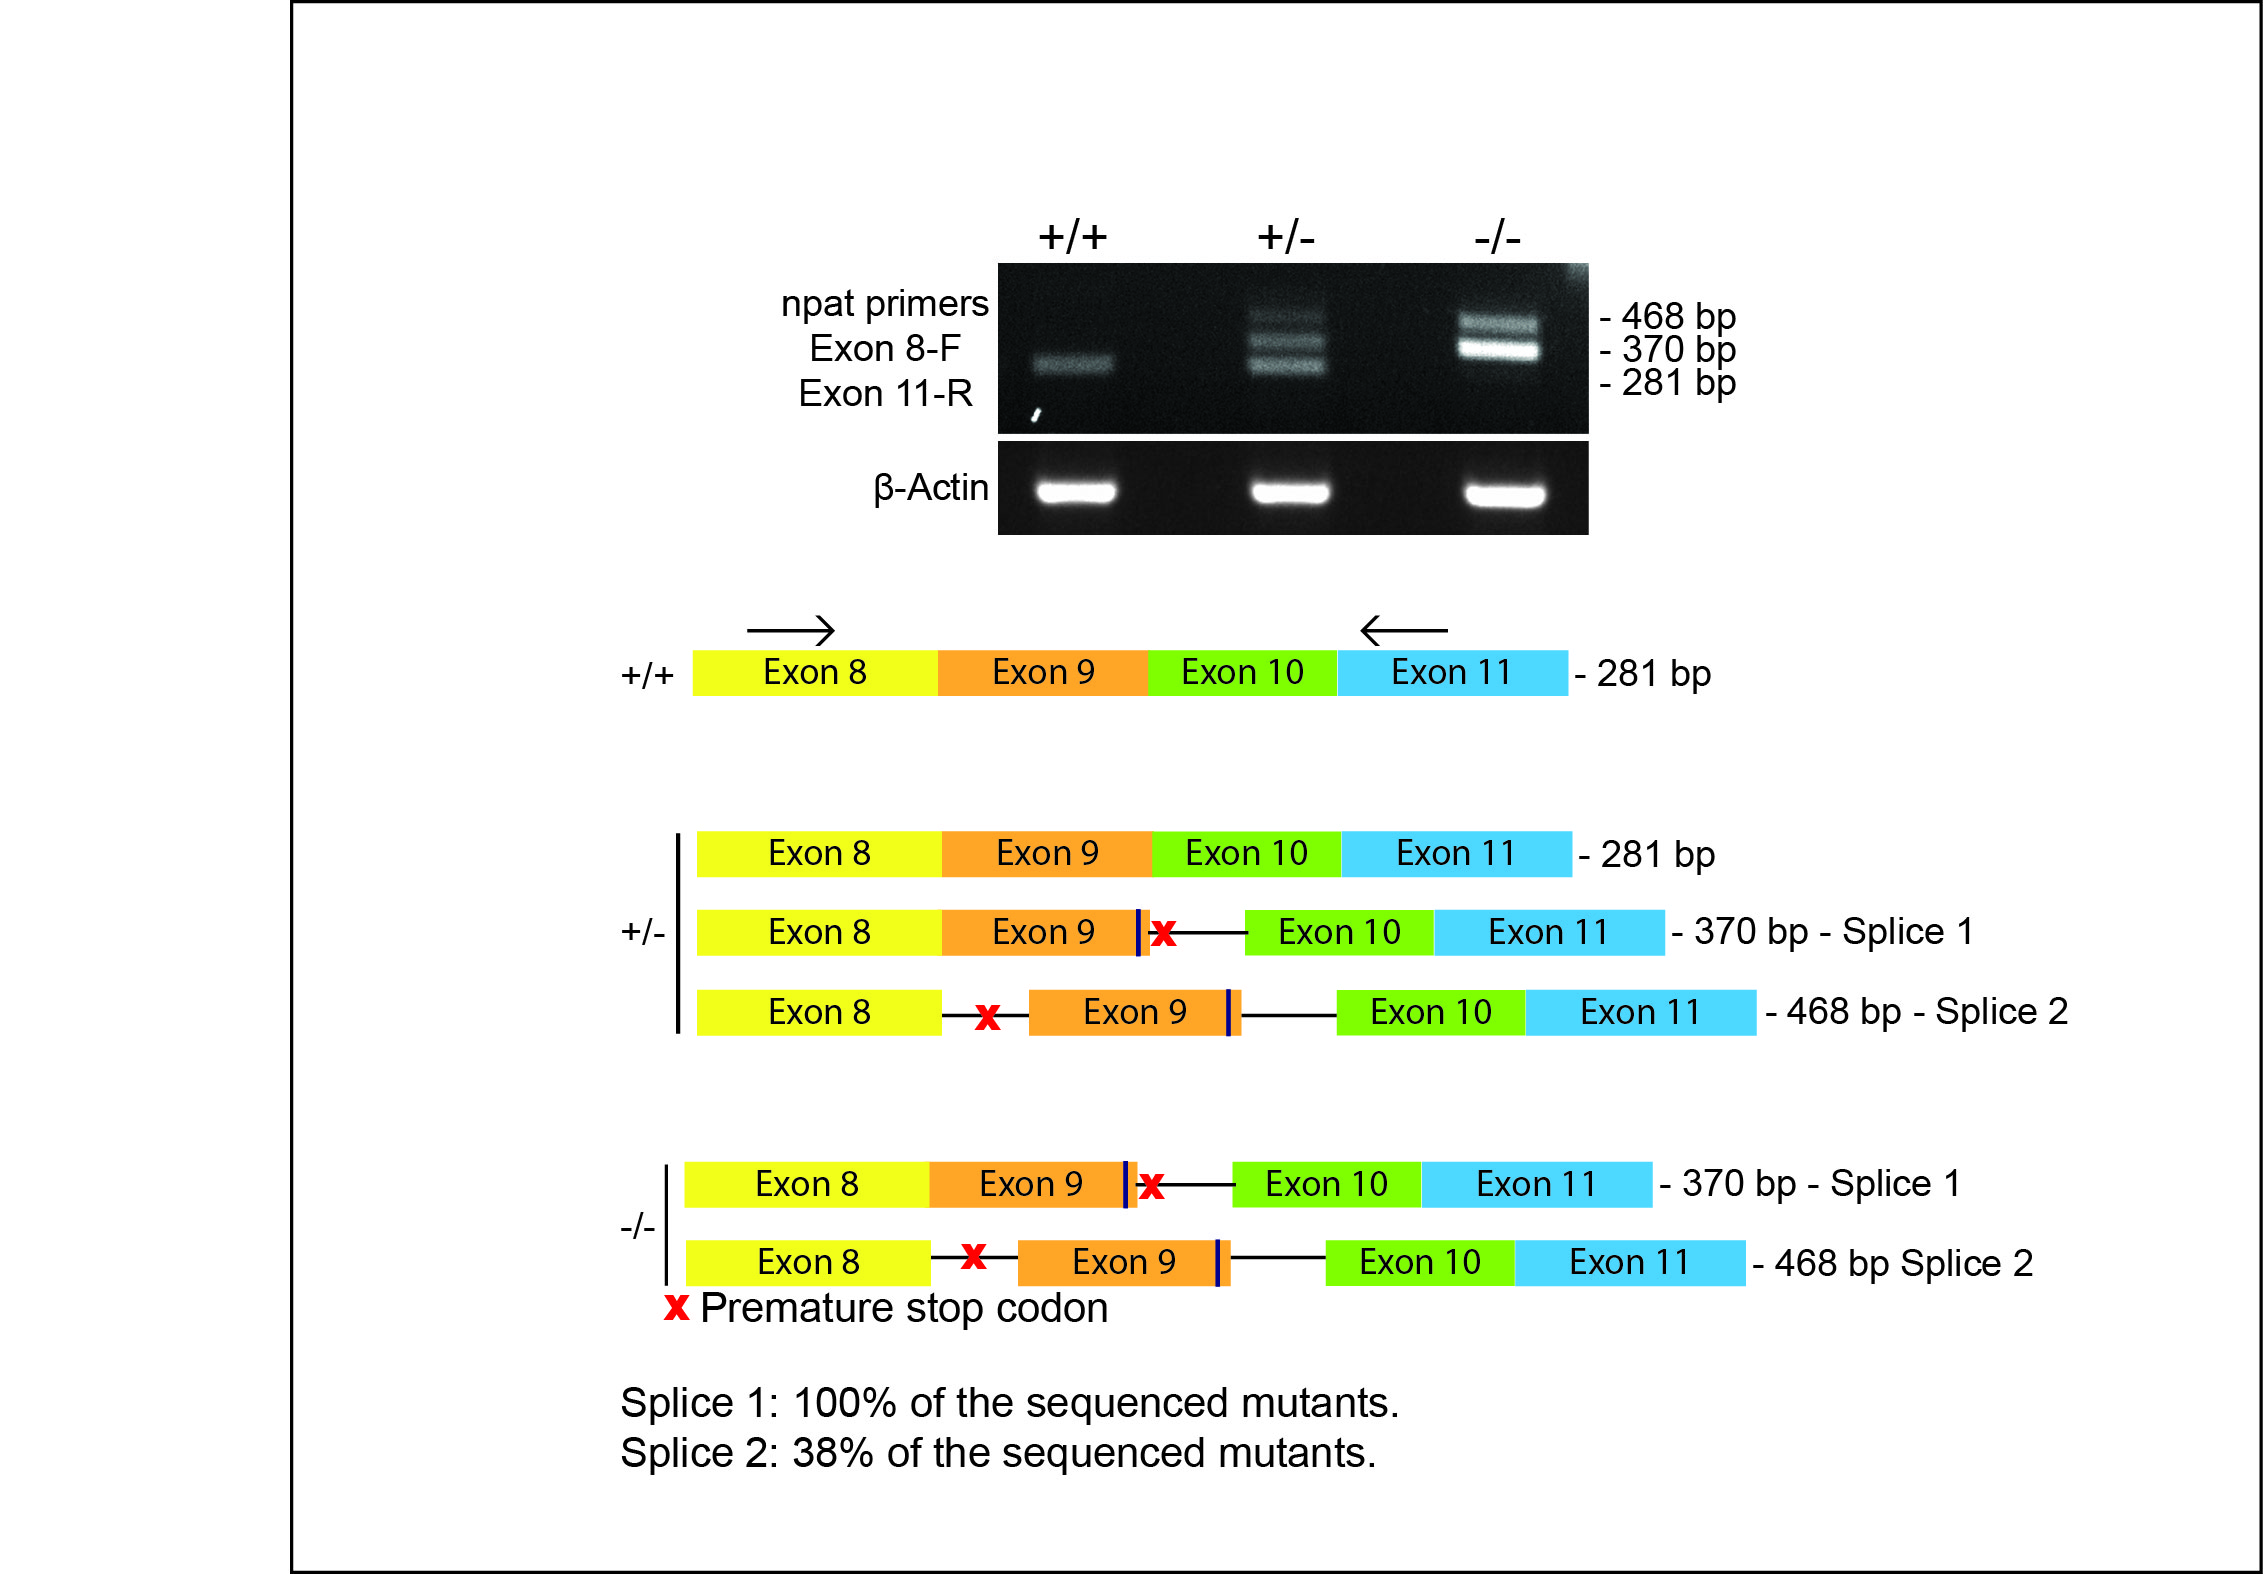
\includegraphics[width=.8\textwidth]{rys/PCRE8-E11WtSibRys.jpg}}    
    \caption{{\bf RT-PCR analysis reveals two aberrant intron retention variants in \textit{rys} mutant npat transcripts}}
    \label{npattranscript}
    Top panel: Agarose gel electrophoresis of mRNAs prepared from 3dpf homozygous wild type (+/+), heterozygote (+/-), and homozygous mutant (-/-) animals, as identified by genomic PCR. Fragments were amplified from a forward primer sited in exon 8 and a reverse primer sited in exon 11.
    Bottom panel: exon/intron layout schematics of the putative transcripts detected.
\end{figure}

\begin{figure}[!h]
    \makebox[\textwidth][c]{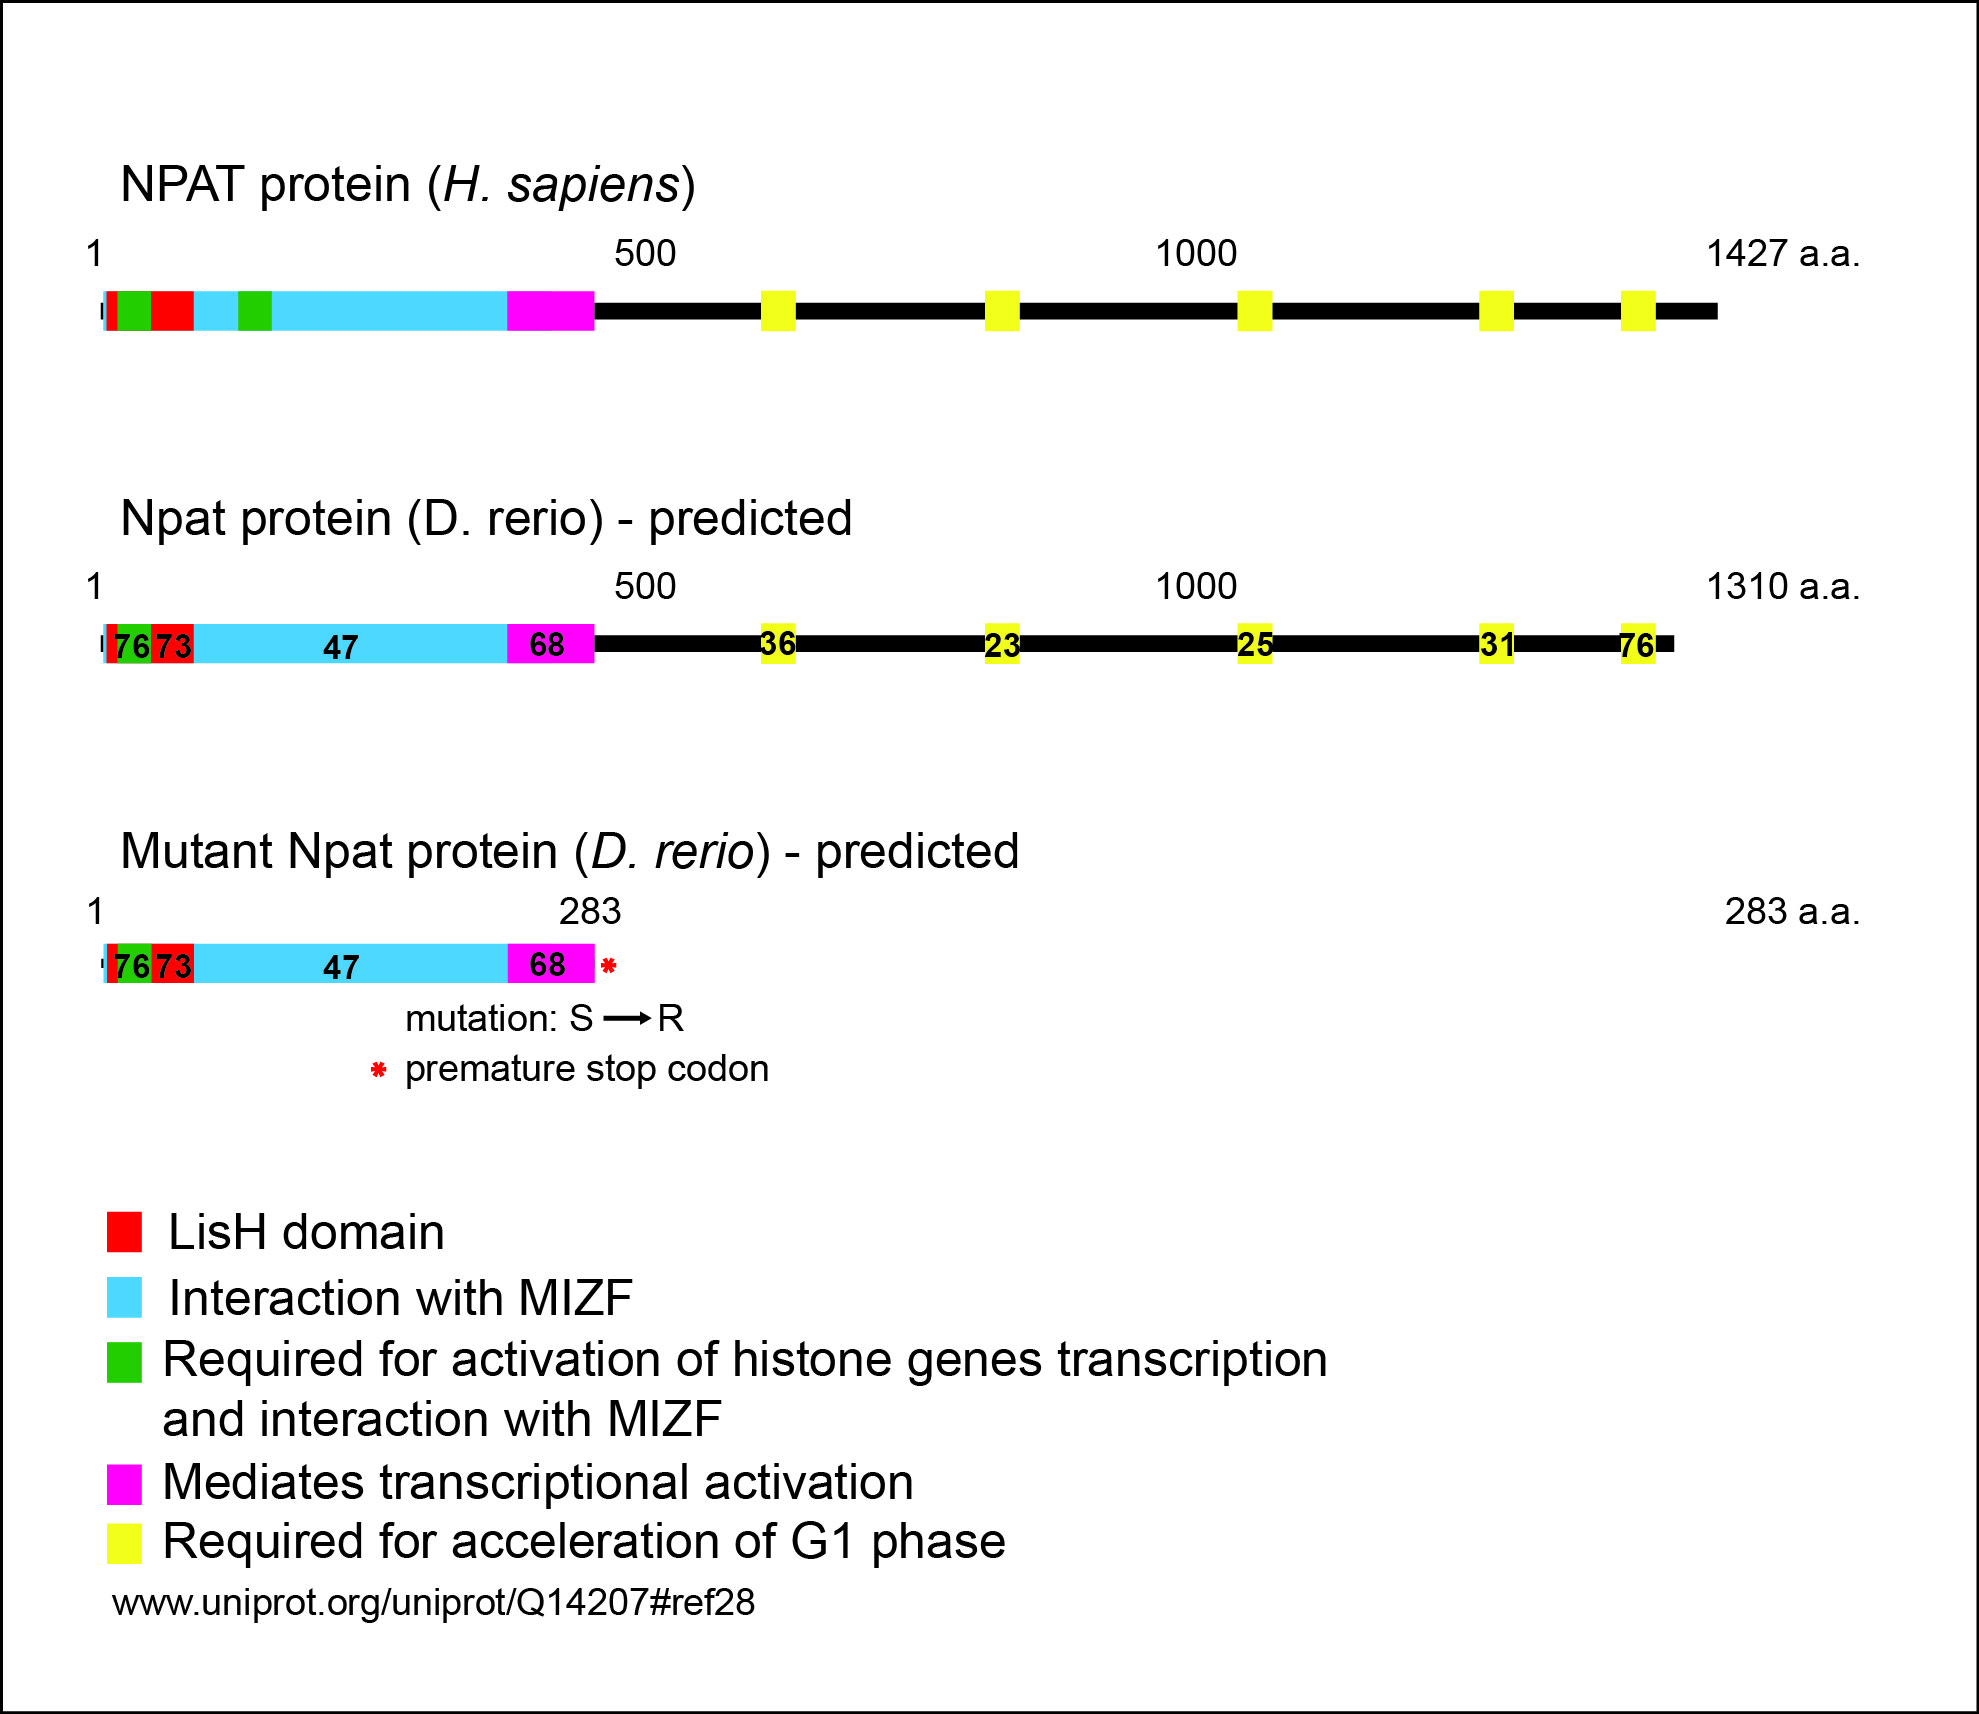
\includegraphics[width=.8\textwidth]{rys/Npat protein.jpg}}    
    \caption{{\bf Functional domains of Human NPAT compared to predicted wild-type and \textit{rys Danio} npat}}
    \label{npatprotein}
\end{figure}
\FloatBarrier

Because \textit{D. rerio} is a teleost known to have undergone genome duplication in an ancestral clade, we used the Synteny Database tool \cite{Catchen2009} identify any possible duplicates; plausibly, a duplication in zebrafish npat could explain the lessened severity of the mutant phenotype when compared to mammalian proviral inactivants. The results of this analysis are presented in Supplementary \autoref{synteny}. While npat is in the midst of a region which appears to be duplicated on chromosomes 5 and 15, relative to the unduplicated homologous syntenic run on \textit{H. sapiens} chromosome 11, it is not, itself, duplicated.

We performed in situ hybridisation using a probe directed to the wild type npat transcript to confirm that the gene is indeed expressed in wild type CMZs; we found that npat expression is progressively restricted to the CMZ from 4 to 6 dpf in wild-type fish. A representative time-course of 20 \si{\micro\metre} cryosections through ISH-treated embryos is depicted in \autoref{npatISH}, focusing on the retina at the times when it has formed. While npat remains transcribed in both the specified GCL and amacrine-rich inner INL to a degree, it is most intensely expressed in the proliferative CMZ, as we might expect on the basis of its cell cycle functions.

\begin{figure}[!h]
    \makebox[\textwidth][c]{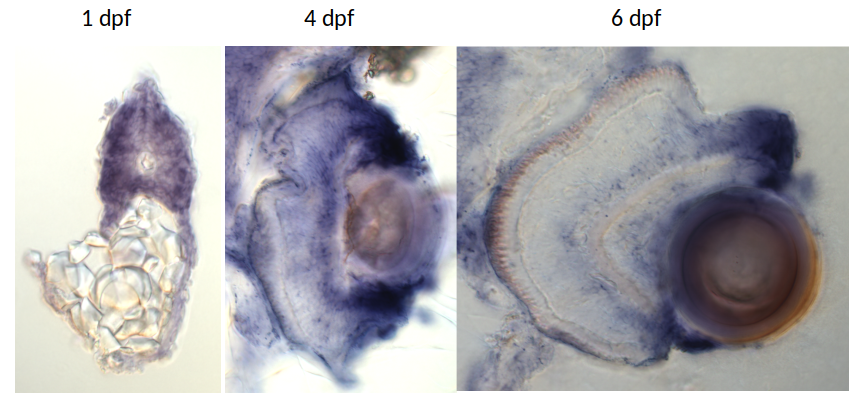
\includegraphics[width=.8\textwidth]{rys/ISH.png}}    
    \caption{{\bf In situ hybridization reveals progressive restriction of npat expression to the CMZ}}
    20\si{\micro\metre} sections of wild-type embryo (1dpf) and retinae (4 and 6 dpf), displaying progressive restriction of npat expression as assayed by in-situ hybridisation.
    \label{npatISH}
\end{figure}

Having taken note of the unusual chromatin ultrastructure present in \textit{rys} CMZ RPCs, and with a mutant npat allele reliably linked to the appearance of the \textit{rys} phenotype, we investigated the transcriptional status of npat and its histone regulatory targets in these animals. We first assayed npat itself by RT-PCR, finding that homozygous \textit{rys} mutants overtranscribe npat by about 3-fold compared to their wild-type counterparts at both 6dpf and 8dpf, while sibling overabundance declines from about 2.5-fold to 1.5-fold over this time period, as shown in \autoref{npatrtpcr}, with calculated marginal posterior mean mass over the WT standard given in \autoref{rtpcrtable}.

Since mammalian NPAT is known to regulate histone transcription and is critical for coordinating the correct expression of replication-dependent histone transcripts required to package genomic DNA during S-phase \cite{Zhao2000}, we hypothesized that the altered nuclear morphology and truncated S-phase we observed in proliferating \textit{rys} CMZ cells may be a consequence of perturbed regulation of histone transcription. To test this, we performed qPCR on random-hexamer-primed cDNAs produced from 6 and 8dpf wild type, sibling, and \textit{rys} embryo mRNA extracts. These qPCR assays were performed using degenerate primers\footnote{Zebrafish have notably populous histone clusters with numerous variants and pseudogenes not present in non-genomically-duplicated vertebrates, so degenerate primers are an appropriate way to survey the population of transcripts. A full catalogue has not been undertaken, to my knowledge.} directed toward all members of the zebrafish core histone gene families H2A, H2B, H3 and H4. As a role for NPAT in 3’ end processing of histone transcripts has been identified \cite{Pirngruber2010}, we also set out to determine whether 3’ end processing of histone transcripts is altered in \textit{rys}. By repeating the above-described qPCR assays on oligo-dT-primed cDNAs, we were able to examine the population of polyadenylated histone transcripts in isolation. 

\begin{figure}[!h]
    \makebox[\textwidth][c]{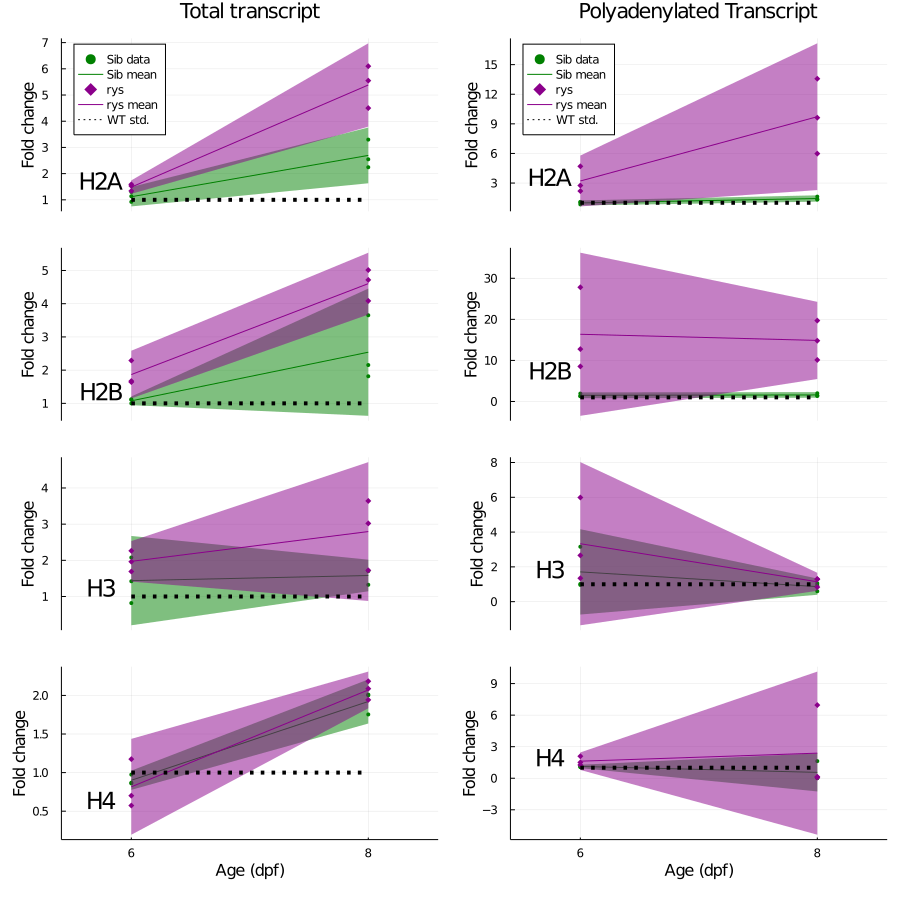
\includegraphics[width=.8\textwidth]{rys/qPCR.png}}    
    \caption{{\bf \textit{rys} overexpress total and polyadenylated core histone transcripts}}
    qPCR results for degenerately-primed families of core histone transcripts, from random hexamer primers for panels A and B, measuring total core histone transcripts, and oligo-dT for panels C and D, measuring polyadenylated transcripts. Panels A and C display results from cDNAs of 6dpf \textit{rys} mutants and siblings compared to wild-type conspecifics, while B and D are from 8dpf animals.    
    \label{histonertpcr}
\end{figure}

To plausibly be implicated in the \textit{rys} phenotype, a candidate histone transcript ought to be overexpressed in mutants relative to both WT and siblings at 6dpf and 8dpf. In order to determine the best-supported candidates for causative involvement in \textit{rys}, we calculated the standard deviations of significance which obtain on the test of mean rys transcript being greater than either mean sibling transcript or the WT standard (set to 1.0). These values are presented in \autoref{qPCRstds}.

\begin{table}[!ht]
    \centering
    \caption{{\bf Standard deviations of significance for \textit{rys} mutant transcript $>$ sib or WT}}
    \begin{tabular}{|l|l|l|l|l|} 
        \hline {\bf Pool} & {\bf Transcript} & {\bf Age} & {\bf Sib mean $\sigma$} & {\bf WT std $\sigma$}\\ \hline 
        Total & H2A & 6 & 1.59 & 3.72\\ \hline
        Total & H2A & 8 & 2.75 & 5.4\\ \hline
        Total & H2B & 6 & 2.12 & 2.37\\ \hline
        Total & H2B & 8 & 1.9 & 7.59\\ \hline
        Total & H3 & 6 & 0.77 & 3.39\\ \hline
        Total & H3 & 8 & 1.21 & 1.83\\ \hline
        Total & H4 & 6 & -0.26 & -0.58\\ \hline
        Total & H4 & 8 & 0.79 & 8.83\\ \hline
        polyA & H2A & 6 & 1.68 & 1.68\\ \hline
        polyA & H2A & 8 & 2.18 & 2.3\\ \hline
        polyA & H2B & 6 & 1.47 & 1.52\\ \hline
        polyA & H2B & 8 & 2.76 & 2.89\\ \hline
        polyA & H3 & 6 & 0.6 & 0.97\\ \hline
        polyA & H3 & 8 & 0.78 & 0.54\\ \hline
        polyA & H4 & 6 & 1.15 & 1.46\\ \hline
        polyA & H4 & 8 & 0.45 & 0.35\\ \hline
    \end{tabular}
    \label{qPCRstds}
\end{table}

Following these calculations, we find the greatest significance at 6dpf for the \textit{rys} overexpression of total H2B transcript, followed by polyadenylated H2A, total H2A, and polyadenylated H2B. The ordering for 8dpf is similar: the most significant overexpression results are for polyadenylated H2B, then total H2A, polyadenylated H2A, and total H2B. We note that the overabundances of polyadenylated H2A and H2B are approximately 2-20 fold greater than those observed for any other transcript pool or histone family. 

We assess the joint probability that mean \textit{rys} mutant total H2A is greater than the sib mean at both 6dpf and 8dpf to be 99.7\% $\pm$ 5.0; the same figure for H2B is 98.5\% $\pm$ 5.1. The joint probability that mean total H2A and H2B are elevated in \textit{rys} mutants compared to sibs at both ages is therefore 98.2\% $\pm$ 7.1. For the polyadenylated transcripts, the joint probability that the \textit{rys} mutant polyA H2A mean is greater than the sib mean at both ages is 94.1\% $\pm$ 9.9; the same figure for H2B is 92.6\% $\pm$ 3.3. The joint probability that mean polyadenylated H2A and H2B are elevated in \textit{rys} relative to sibs at both ages is then 87.1\% $\pm$ 9.7. On the basis of these calculations, we suggest the most plausible causal contributor to the \textit{rys} phenotype, of the transcript families examined, are H2A and H2B transcripts. While the relative magnitude of the overabundance of total H2A and H2B transcript is less than that of the polyadenylated pool, we have significantly less uncertainty about these figures. Still, the polyadenylated transcript results seem to speak to a fundamnetal loss of control over the abundance of these gene products; unlike the total transcript pool, siblings retain tight, WT-like control over polyadenylated transcripts, while \textit{rys} mutants display much more extensive variability in polyA transcript expression, even where the mean is not elevated above siblings or WT controls.

\begin{figure}[!h]
    \makebox[\textwidth][c]{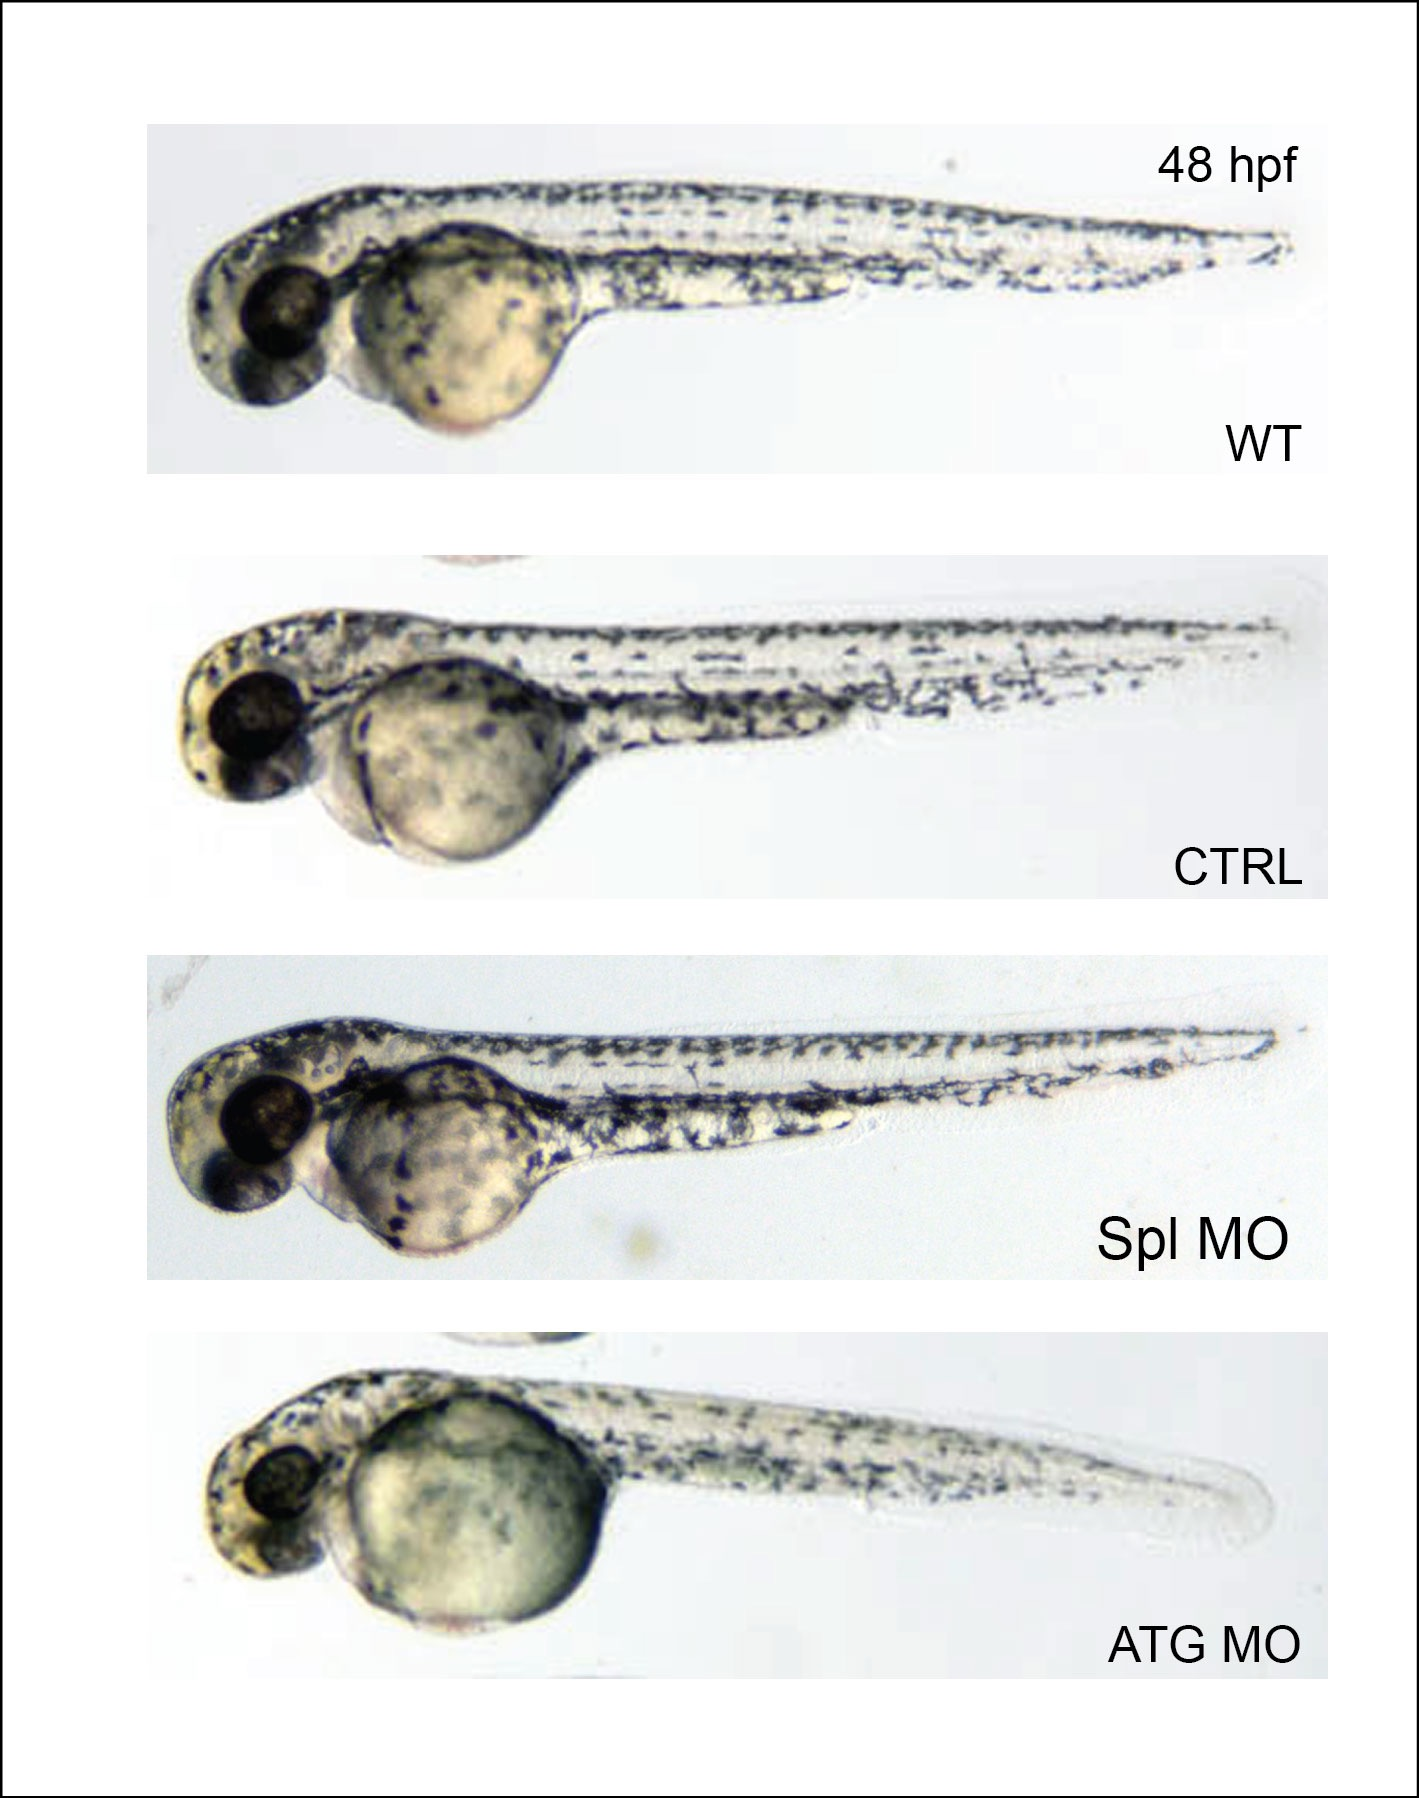
\includegraphics[width=.7\textwidth]{rys/morpholinos.jpg}}    
    \caption{{\bf 48hpf embryos injected with an npat ATG-targeted morpholino display a small-eye phenotype}}
    20\si{\micro\metre} sections of wild-type embryo (1dpf) and retinae (4 and 6 dpf), displaying progressive restriction of npat expression as assayed by in-situ hybridisation.
    \label{morpholinopics}
\end{figure}

While these observations substantiate the involvement of npat in the \textit{rys} phenotype, we pursued the matter further by perturbing npat using morpholino injections of wild-type fish. As we do not suppose morpholino transcriptional blockade will precisely replicate the cellular conditions of a genetic null some days after birth, we did not seek to recapitulate the \textit{rys} phenotype. Rather, we sought to determine if any of \textit{rys}'s constituent phenomena would appear after an early blockage of \textit{rys} transcription, further substantiating the general involvement of npat in \textit{rys}. We tested morpholinos directed both to the npat start codon and to the splice site affected in \textit{rys}, alongside control morpholinos and uninjected animals. We used both a morpholino directed to the transcript ATG start site, as well as to the affected splice site. The splice morpholino consistently replicated the \textit{rys} phenotype on both total and polyadenylated core histone transcript abundance, while the ATG morpholino more narrowly replicated the effect on polyadenylated transcript (\autoref{morpholinoRTPCR}). The ATG morpholino produced animals with small eyes by 72dpf, as shown in \autoref{morpholinopics}, and confirmed by census of the cellular population of central coronal sections through the retina \autoref{morpholinonuclei}. These results establish that the identification of npat as the causative mutation in \textit{rys} is plausible, as experimental perturbation to npat in WT fish can cause \textit{rys} phenotypic phenomena. 

\subsection{\textit{rys} siblings and mutants have unique sets of nucleosome positions, best explained by different sequence preferences and increased sequence-dependent positioning in mutants}
 Our observation of perturbed histone expression in \textit{rys} embryos led us to suspect that the aberrant nuclear morphology observed in \textit{rys} CMZ progenitors arises from disrupted chromatin organisation, which is a possible consequence of altering the dynamic composition of the histone pool available for nucleosome formation during cell cycle. We therefore sought to characterise nucleosome positioning in \textit{rys} and wild-type siblings by micrococcal nuclease (MNase) digestion of pooled genomic DNA (gDNA). Nucleosome-protected fragments from the MNase digests were sequenced and positions called as described previously.


 \begin{figure}[!h]
    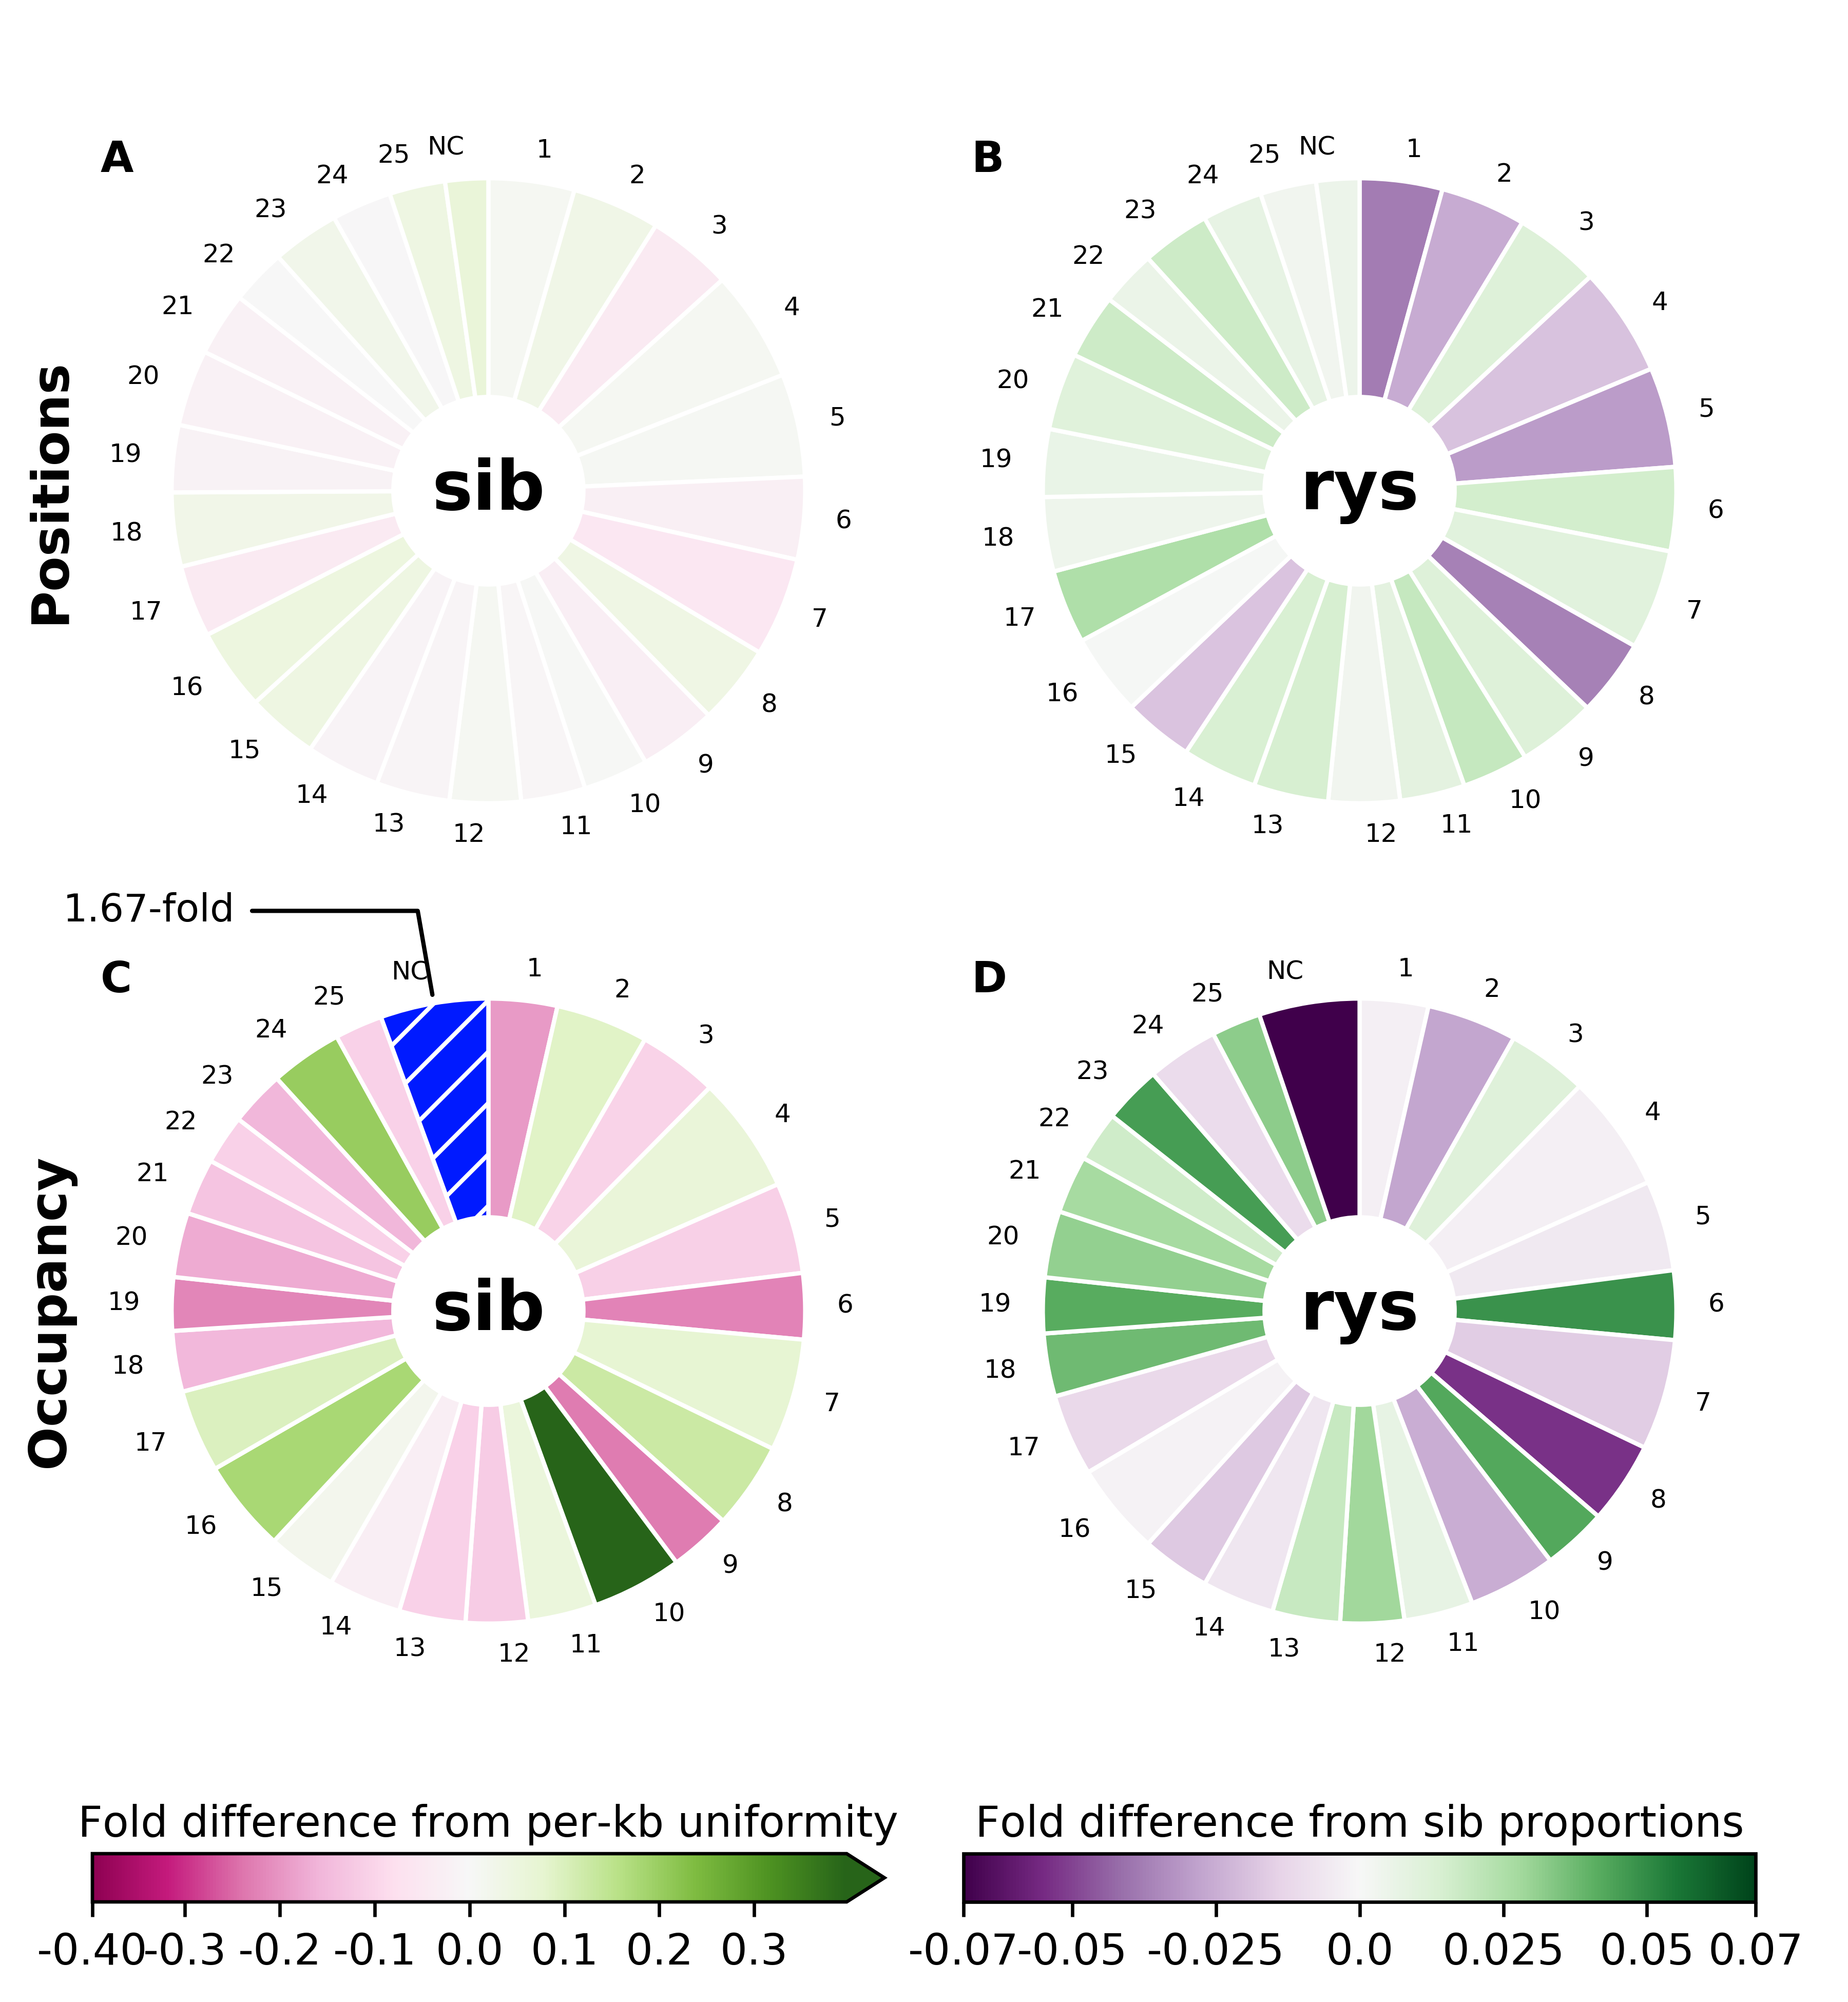
\includegraphics{rys/proportional_chromosome_occupancy.png}
    \caption{{\bf \textit{rys} chromosomes are differentially enriched and depleted of nucleosome position density and occupancy.}}
    Pie charts of nucleosome position density and occupancy by chromosome. Width of pie slices in panels A and B indicates the fraction of the total number of positions occuring in the numbered chromosomes and nonchromosomal scaffolds (NC). In panel A, depicting the sib genome, slices are colored according to the extent of deviation from an assumption of even distribution of nucleosomes across the genome. In panel B, depicting the \textit{rys} genome, slices are colored according to the extent of deviation from the sib distribution. The width of slices in slices B and D indicate the fraction of the total nucleosome occupancy signal detected. Slice coloration depicts deviations from nucleosome occupancy distributions analogous to position distributions in A and B. Blue and white diagonal bars in the NC slice of panel C denote an out-of-scale positive deviation from the assumption of even distribution, i.e., sib NC scaffolds have 1.67-fold more of the total nucleosome occupancy signal than is expected from their length alone.  
    \label{nucgendist}
    \end{figure}
    
 We first examined the genomic disposition of nucleosome positions within wild-type siblings and \textit{rys}. We found nucleosome positions distributed relatively evenly over sib genomic material, with only tiny deviations from a neutral assumption of a uniform distribution of the total position number over the full length of the genome, as displayed in Fig. \ref{nucgendist}, panel A. Bulk \textit{rys} chromatin displays minor differences from the proportions of positions found in each sib scaffold (panel B). Sib nucleosome positions are differentially occupied across scaffolds, with Chr 10 and scaffolds not yet mapped to chromosomes (NC) being notably more occupied than expected from scaffold length alone (panel C). Similarly to the distribution of positions, \textit{rys} chromatin is somewhat more evenly occupied than sibs; scaffolds with positions that are more heavily occupied in sibs tend to be depleted in \textit{rys} and vice versa (panel D). 


\begin{figure}[!h]
    \makebox[\textwidth][c]{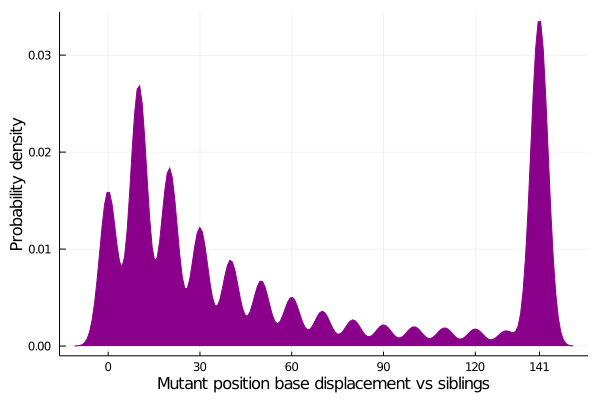
\includegraphics[width=.75\textwidth]{rys/shiftdist.png}}    
    \caption{{\bf PWM sources detected in sibling differential nucleosome positions.}}
    Probability distribution of \textit{rys} position displacement distance from mapped sibling positions, in base pairs. 
    \label{shiftdist}
\end{figure}

By mapping the called nucleosome positions in rys to those in sibs, and calculating the number of bases the \textit{rys} position is displaced from its mapped position, we characterised the population of \textit{rys} positions by translational displacement from the arrangement found in siblings. The probability distribution of this displacement parameter for the population of \textit{rys} positions is displayed in \autoref{shiftdist}. The notable bimodality of this distribution arises as a result of the inclusion of unmapped positions, to show the relative size of this population: 23\% of positions are not mapped to any sibling position at all; these are located at 141, the full length of a called nucleosome position in our pipeline. The other three-quarters of the positions are mapped to sibling positions, with 11\% of overall \textit{rys} positions coinciding entirely with the sibling positions, 19\% displaced 10 bases or less from a sib position, and a further 21\% displaced between 10 and 30 bases. The last quarter of \textit{rys} positions display more extreme displacements, up to the entire length of the position. The periodic multimodality observed in the displacement distance of \textit{rys} positions relative to sibs is commonly observed in patterns of nucleosome positioning and arises from the 10-base perioicity of nucleosome contacts with DNA \cite{Wright2017}. This distribution of population displacement strongly suggests that the npat mutation in \textit{rys} results both in a loss of translational control of nucleosomes that are in approximately the expected positions, most commonly by a nucleosome ``roll''of one contact, as well as a loss of trans-acting nucleosome positioning control which gets nucleosomes to the correct positions to begin with, represented by the novel \textit{rys} positions, with no mapped sibling ounterpart.

Mindful of the whole-organism source of the nucleosomal genomic sample used to generate the called positions, and of the heterogenous nature of the \textit{rys} phenotype, with RPCs displaying the nuclear phenotype but not specified retinal neurons, the second, novel, group of positions mentioned above was of interest, as we sought to identify position subpopulations that might represent those involved in the nuclear phenotype. Interestingly, not only are there \textit{rys} nucleosome positions which are not found in siblings, but there is likewise a subset of sib positions which are never found to be occupied in rys . Intriguingly, sib positions which are not observed in rys are compensated for quite evenly across the genome by new positions gained in the mutants, with a small excess of new rys positions on most chromosomes, as shown in Supplementary \ref{diffposdist}.

This result suggested that a particular subpopulation of wild type nucleosomes are mislocalised in \textit{rys}. If the pool of available histones in proliferating \textit{rys} progenitors is substantially different from that of siblings, \textit{rys} nucleosomes forming from this pool may have altered physico-chemical interactions with DNA, which could result in a preponderence of nucleosomes with unusual sequence preferences. If so, this would explain the disappearance of a subset of positions in \textit{rys} and the appearance of a new, similarly sized subset of positions (the `differential set').

To formally address this hypothesis, we calculated the Bayesian evidence ratio for separate emission processes for sib and \textit{rys} position sequences against a combined process for both sets of sequences. If the molecular process resulting in the differential set arises from altered nucleosome composition in proliferating \textit{rys} cells, we expect these sequences to provide greater support for separate emission processes than for a single, combined process. On the other hand, if abberant DNA-nucleosome interaction is not causally relevant, and the reason for the apparently displaced nucleosomes is another macromolecular process, the evidence ratio should favour a combined process for the emission of the differential set- that is, there should be no difference between the unique sib and \textit{rys} sequences that would justify the additional complexity of separate models.

The emission model used was the Independent Component Analysis form described by Down and Hubbard \cite{Down2005}, with a fixed number of independent, variable length position weight matrices related to observations by a Boolean mixing matrix. An observation is scored by the background likelihood of its sequence, given some model of genomic noise, convolved with a sequence-length- and cardinality-penalized score\footnote{That is, the additional score provided by a source to an observation is penalized both by the expected number of motif occurrences given an observation of that length, as well as by the number of sources which explain the observation in the model.} for each source which the mix matrix indicates is present in the observation. Therefore, we first needed to construct background models of \textit{D. rerio}'s genomic "noise" from which repetitive sequence signals characteristic of nucleosome positions could be extracted. Following the suggestion of Down and Hubbard \cite{Down2005} that a principled approach to the selection of background models is to train and test a variety of them on relevant sequence, we used the Julia package BioBackgroundModels (presented in \autoref{ch:BBM}) to screen a panel of 1,2,4, and 6-state HMMS against  0th, 1st, and 2nd order encodings of samples from the zebrafish genome, partitioned grossly into exonic, periexonic, and intergenic sequences. We found that each of these partitions is best represented by 6-state HMMs trained on a 0th order genome encoding (i.e. the HMMs emit the 4 mononucleotides), as determined by model likelihood given an independent test sample, as displayed in \autoref{BHMMlh}.

We next used the Julia independent PWM component analysis nested sampling library BioMotifInference (presented in \autoref{ch:BMI}) to sample from the posterior distribution, given the differential set of \textit{rys} nucleosome positions and the composite background model of genomic noise. We initialized separate ensembles from uninformative priors on the \textit{rys} and sib data alone, as well as the combined \textit{rys} and sib data, allowing for 8 independent PWM sources in all cases. We compressed three model ensembles to within 125 orders of magnitude between the maximum likelihood model sampled and the minimum ensemble likelihood\footnote{That is, the convergence criterion was that the ensemble difference $log(L_{max})-log(L_{_min}$ be <125).}. This process produced the model evidence estimates summarized in \autoref{BMIevidencetable}, as well as maximum a posteriori samples for each of the ensembles. We estimate that there are orders of magnitude of evidence in favour of separate generative processes for the differential sib and \textit{rys} than for a combined model, with an estimated standard deviations of significance. We present the MAP PWM source samples from the better-evidentiated separate \textit{sib} and \textit{rys} models in \autoref{sibmotifs} and \autoref{rysmotifs} respectively, while the inferred combined sources are available in Supplementary \autoref{combinedmotifs}.

BioMotifInference's source detection was highly conservative, likely due to the good quality of the background models, which were found to explain a majority of observed nucleosome positions adequately without any PWM sources in most models of the maximum a posteriori estimate for both sibling and rys ensembles. In siblings, the top three sources are the only ones detected in more than 10\% of observed sequences, suggesting that the influence of sequence preferences is weakly explanatory for these sites. By contrast, we found twenty-eight separate PWM sources expressed in more than 10\% of observations, in a variety of posterior modes. This suggests sequence preferences are much more explanatory for the \textit{rys} differential position set.

The detected sources in the siblings are not altogether unexpected; CWG motifs are among the most commonly reported in nucleosome sequences, and have been described as promoting nucleosome formation. The majority of the sources detected in the various posterior modes were of this form, with rarer CT- and CA- dinucleotide repeats, as well as an rare ATGG repeat. \textit{rys} positions have a much more diverse set of sources detectable above background genomic noise; notably, AG- dinucleotide repeats that are not found in \textit{sib} sources at all. The CWG motifs also exhibit a preference for flanking A positions that is not evident in the sibling differential position set. CA- dinucleotide repeats are more commonly detected in \textit{rys} positions, and the rare ATGG repeat is not found at all.

\begin{figure}[!h]
    \makebox[\textwidth][c]{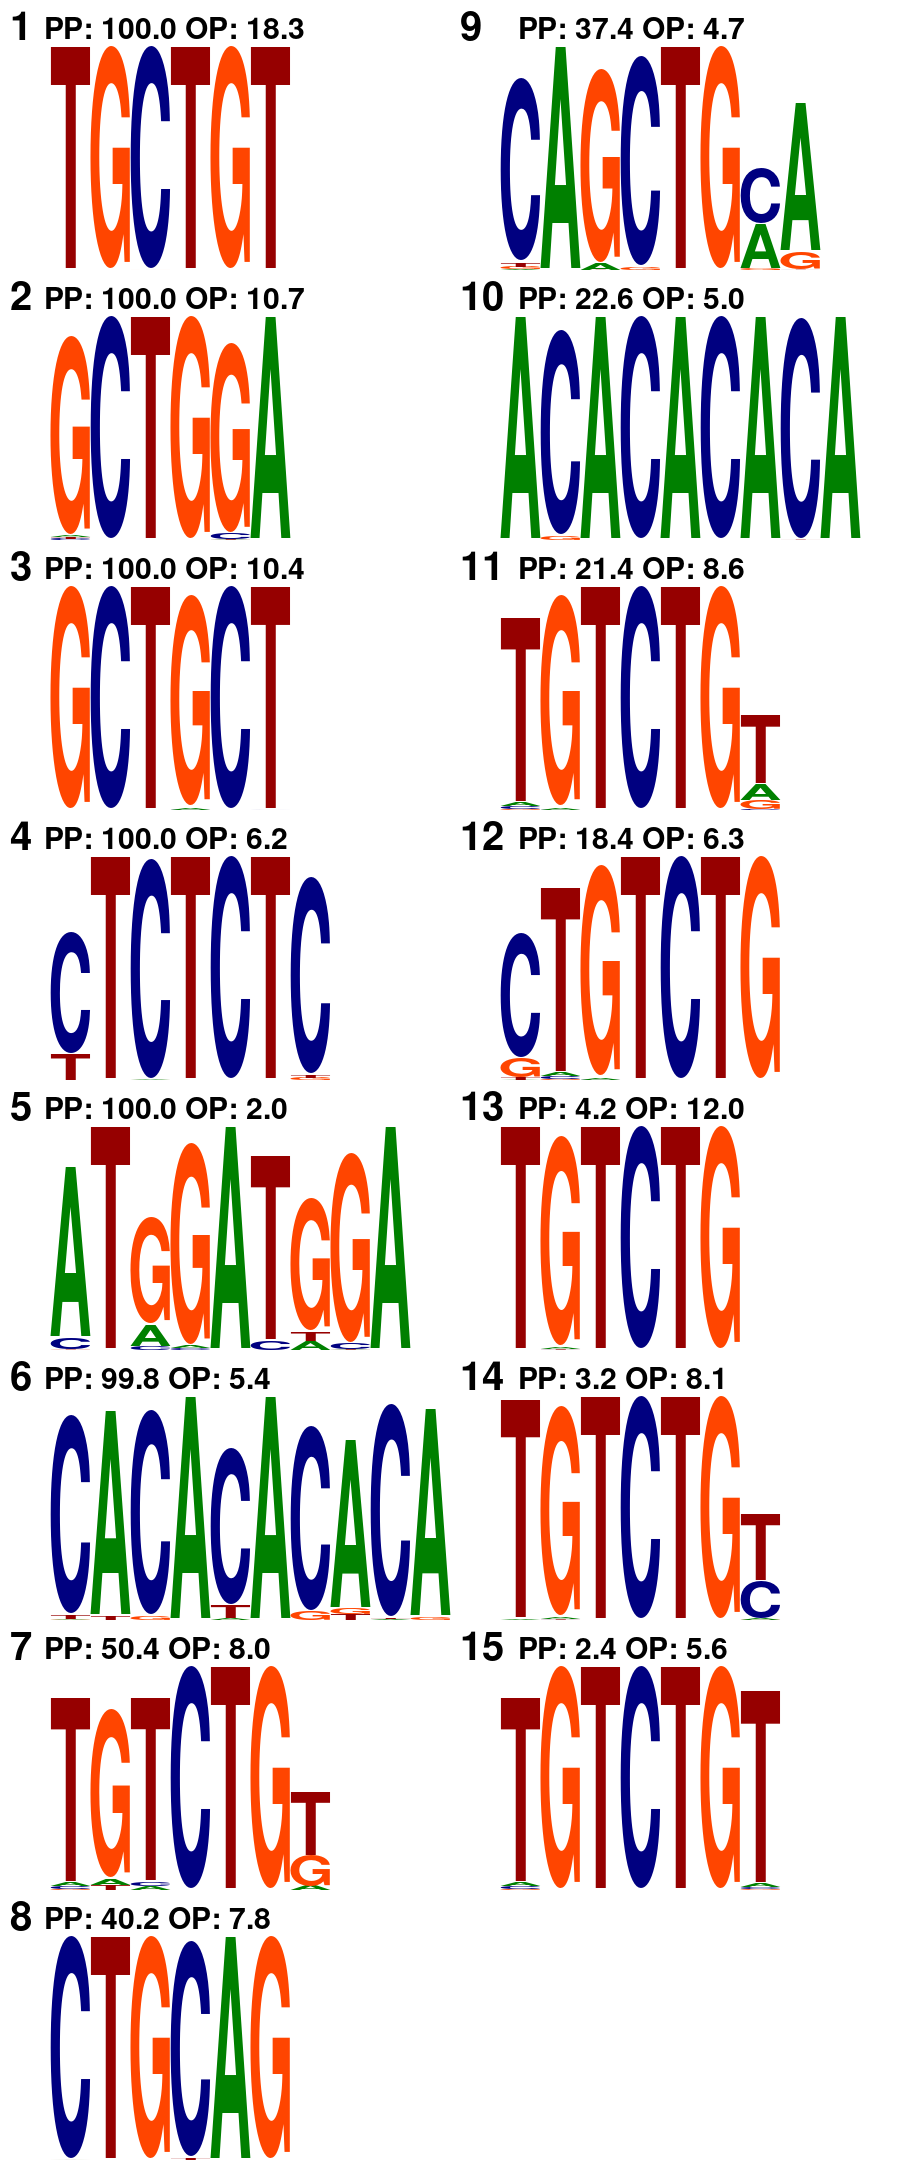
\includegraphics[width=.5\textwidth]{rys/sib_e_srcs.png}}    
    \caption{{\bf PWM sources detected in sibling differential nucleosome positions.}}
    Counts of positions found in sib but not \textit{rys} (red bars, represented as negative numbers, as these are `lost' in \textit{rys}) and those found in \textit{rys} but not sib (blue bars, `gained'). The magnitude of the difference between the counts is represented with a yellow bar.
    \label{sibmotifs}
\end{figure}

\begin{figure}[!h]
    \makebox[\textwidth][c]{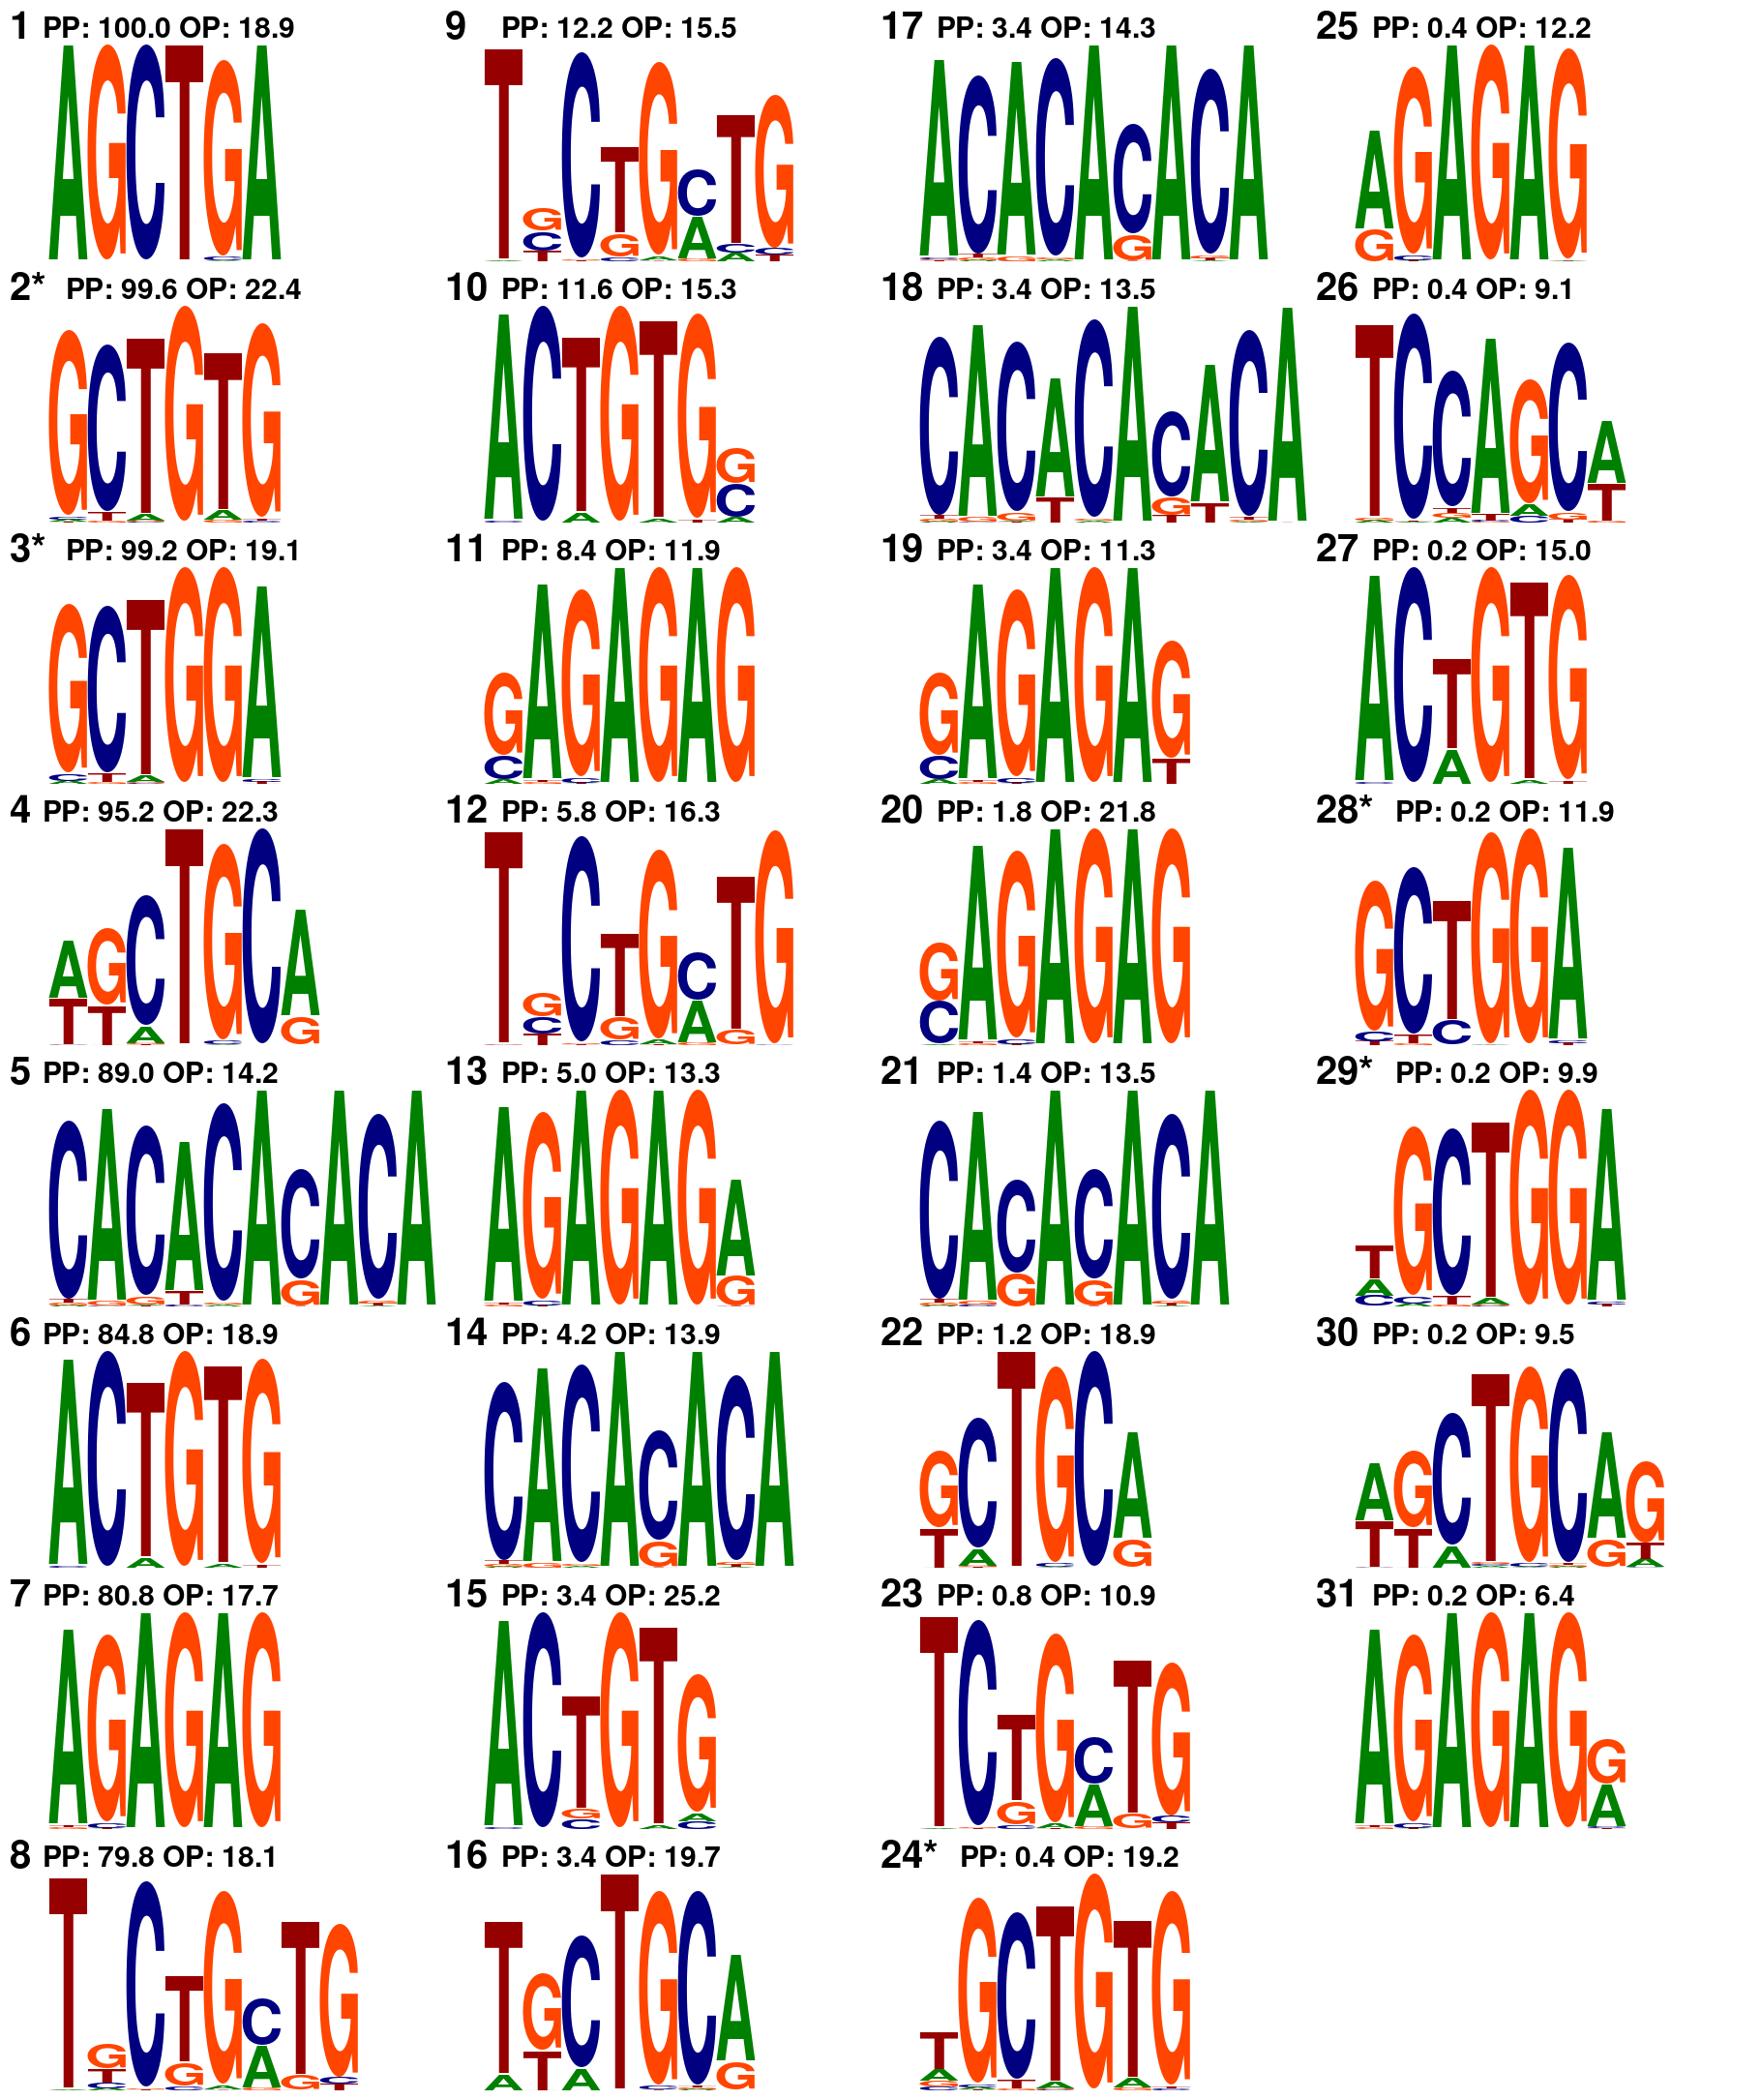
\includegraphics[width=1.\textwidth]{rys/rys_e_srcs.png}}    
    \caption{{\bf PWM sources detected in \textit{rys} mutant differential sources.}}
    Counts of positions found in sib but not \textit{rys} (red bars, represented as negative numbers, as these are `lost' in \textit{rys}) and those found in \textit{rys} but not sib (blue bars, `gained'). The magnitude of the difference between the counts is represented with a yellow bar.
    \label{rysmotifs}
\end{figure}

\FloatBarrier

\section{Discussion}
We began our investigations by adding depth to the original description of the \textit{rys} mutant CMZ phenotype; on the basis of these investigations, we believe that a revision is in order. At any given time, the apparently increased size of the CMZ in \textit{rys}, relative to siblings, is produced as an effect of one or more of the following phenomena:

\begin{enumerate}
\item\label{inapret} Inappropriately retained RPCs in animals older than 7dpf
\item\label{specfail} Reduced neural population of the specified central retina, relative to the CMZ
\item\label{chromo} Expanded and spread-out RPC nuclei
\end{enumerate}

The first two effects are consistent with a failure of RPCs to specify as particular retinal neural lineages. This is substantiated by the inappropriate retention of early progentior markers in these cells. We demonstrate that \textit{rys} RPCs are not, however, arrested in cell cycle. In contradistinction to results finding elevated polyadenylated histone transcript levels associated with cell cyle arrest \cite{Kari2013}, we find that the mitotic activity of these cells actually accelerates under an overabundance of polyadenylated H2A and H2B transcript. We therefore suggest that the \textit{rys} phenotype is best characterised by chromatin disorganisation (phenomenon \ref{chromo}) and a failure of RPCs to correctly specify (which covers phenomena \ref{inapret} and \ref{specfail}) as retinal neural subtypes. The enlarged appearance of the CMZ is a result of these effects, and not a general increase in the CMZ population, RPC cytoplasmic volume\footnote{That is, by itself, without an increase in nucleus size. We did not directly measure this parameter.}, or other variables. 

Moreover, in identifying npat as the lesioned gene underlying the \textit{rys} phenotype, we nominate a general, well-evidentiated macromolecular mechanism underlying phenomenon \ref{chromo} which could plausibly produce phenomena \ref{inapret} and \ref{specfail}. That is, the mutant npat's effects on cell-cycle dependent histone transcription and stability may result in abberrant nucleosome positioning within proliferating cells, by altering the pool of histone proteins available for nucleosome formation. We posit that this is what causes the observed loss of a subpopulation of sibling nucleosome positions in \textit{rys}, together with the gain of novel, abberant positions. When we investigated whether the sequences of these subpopulations were better modelled by separate emissions processes than a combined emissions process, we found substantial evidence in favour of separate emissions processes. Interestingly, the PWM signals we detected in this differential nucleosome position set suggest some detail as to how changes in histone expression might result in the observed nuclear disorganisation of \textit{rys}. The observation that the background models explain the positions unique to siblings better than those unique to mutant \textit{rys} strongly suggests that sequence preference is less important in the process generating sibling positions than in the one generating mutant positions.

The relative importance of primary sequence in nucleosome positioning has been hotly debated; some have advocated for a nucleosome positioning code intrinsic to primary sequence \cite{Kaplan2009}, while others have disavowed the existence of any such code \cite{Zhang2009}. In general, the nucleosome dynamics community has moved on from these discussions in favour of emphasis on rotational sequence preferences \cite{Tolstorukov2007} and translational nucleosome positioning by \textit{trans}-acting factors \cite{Klages-Mundt2018}; a common interpretation of the earlier debate is that sequence preferences tend to dominate only at limiting concentrations of histones, when chromatin formation is rare \cite{Pointner2013}. The fact that sequence preference is less explanatory for the sibling positions than for the mutant ones is highly suggestive against this background. It seems likely that the shifted and novel nucleosome positions observed in mutants reflects all of the following:

\begin{enumerate}
    \item The appearance of nucleosomes with aberrant subunit composition
    \item A loss of translational control over \textit{rys} mutant nucleosomes by \textit{trans}-acting factors
    \item The limiting concentration of aberrantly-expressed nucleosomes, resulting in increased influence of ``default'' sequence-preference positioning
\end{enumerate}

All of the above could plausibly be caused by perturbed histone expression arising from altered npat activity. As the spatiotemporal dynamics of chromatin architecture are known to be critically involved in both replication timing \cite{Gilbert2010} and cell identity and fate \cite{Serrano2013}, the significant alterations we observe in \textit{rys} mutant chromatin architecture also provide a plausible molecular mechanism by which mutated npat protein can produce the observed shift in proliferative activity and failure of RPCs to specify, via altered histone expression. Moreover, chromatin density has recently been specifically implicated as fundamentally involved in the process by which pluripotent cells restrict gene expression to achieve their stable specified fates \cite{Golkaram2017}; it seems to be this overall process which has been disrupted in mutant \textit{rys}.

It is possible that the sequence-level inference is compromised by the ad-hoc nature of the sampler used to compress the ICA ensembles in our nested sampling procedure. For reasons explained in \autoref{ch:BMI}, the ICA model structure makes euclidean space representations difficult, and ensuring sampling is in detailed balance may not be possible, given changing PWM signal lengths. We suggest that it is appropriate to magnify our error estimate by several of magnitude as a consequence. If we concede that there are perhaps 5 orders of magnitude more error than estimated, this has the effect of reducing the significance of the result from to standard deviations, which is still well above the typical 5$\sigma$ significance typically accepted as a discovery in the physical sciences. We conclude that even given a more conservative estimate of the sampling processes' error, it is far more likely that the differential nucleosome populations found in \textit{rys} mutants and their phenotypically normal siblings are the result of separate generative processes. It is also possible that our identification of the differential subset of nucleosome positions with the disordered chromatin present in \textit{rys} RPCs is inaccurate. We have not conducted a full survey of \textit{rys} proliferative niches, and it is not clear how widely affected other cell types might be. Still, within the retina, only proliferative cells seem to have the chromatin phenotype, and it is on this basis that we make the identification, which is the most parsimonious available. 

There are a number of important lacunae in this explanation; it remains unclear what form of the npat protein is expressed, if any, as well as what the overall effect on the expressed pool of histones in RPCs is, for instance. It would not be very surprising if there are a number of macromolecular species intimately invovled in the \textit{rys} pathology which intermediate between the npat lesion and the observed chromatin phenotype which we have not examined. We suggest, however, that the overall effect on specification must be due to a failure of RPCs to organize chromatin for specification, and that, interestingly, this failure does not prevent proliferation. \textit{rys} therefore presents a useful model of the dissociability of proliferative and specificative behaviours in neural progenitors, which has recently been documented elsewhere in the developing \textit{D. rerio} retina \cite{Engerer2017}. Given the methodological limitations we encountered in probing protein expression in \textit{rys} RPCs, we suggest the most interesting and productive avenues of research to pursue in \textit{rys} pertain to this chromatin organisation phenotype.  Further experimentation is required to determine how specific changes in chromosome organisation (e.g. alterations in 3-dimensional chromatin organisation of gene expression, number of replication foci, etc.) produce specific features of the \textit{rys} phenotype. 

The zebrafish \textit{rys} mutant model provides a heretofore unique opportunity to study the role of a human NPAT homologue in a complete, developing tissue. This has previously proven difficult using mouse Npat, proviral inactivation of which resulted in early embryonic arrest, prior to tissue formation (Di Fruscio1997). The survival and development of \textit{rys} mutant embryos beyond this stage may reflect the presence of wild-type npat transcript contributed maternally \cite{Harvey2013}; \textit{rys} mutants nevertheless do not survive beyond metapmorhosis (\textasciitilde{}21dpf), so npat seems to be similarly obligatory for normal development in zebrafish, if over a longer timeframe. Still, we observed many differences between the function of npat in zebrafish and documented effects in other vertebrates, which require some explication.

As teleost fish are known to have undergone whole-genome duplication subsequent to their radiation from vertebrates, it is possible that zebrafish may have multiple npat paralogues. We have excluded this possibility due to our failure to identify any significantly similar CDS sequences in the Zv9 zebrafish genome using BLAST, and the synteny analysis in \autoref{synteny}. The zebrafish npat gene does have a substantially different genomic context from human NPAT, however: it is not associated with the eponymous ATM locus (which has been duplicated, and is present in this duplicate form elsewhere on chromosome 15). ATM’s 5’ position is, in zebrafish, occupied by hif1al, with the intergenic region lacking canonical E2F promoter sites. Of the 80 vertebrate genomes currently available from Ensembl, this organisation is shared only with the cave fish (A. mexicanus), with the human-like ATM-NPAT association preserved in all other species. This apparently evolutionarily novel genomic organisation for npat may be responsible for some of the differences in npat function we report here, relative to its homologues.

We identified alterations in histone mRNA transcription and 3’ end processing as likely mechanistically involved in the \textit{rys} phenotype. In both 6 and 8 dpf \textit{rys} larvae as well as npat-morpholino treated 1dpf embryos, we observe increased abundances of histone and, specifically, polyadenylated histone transcripts, although the composition of affected histone families differs between these contexts. The specific mechanism by which these effects are produced in \textit{rys} remains unclear, and the increases in histone transcript abundance observed in both mutant and morpholino-treated animals is at odds with observations that NPAT knockouts display decreases in histone transcription \cite{Ye2003}, and that the destruction of CDK phosphorylation sites on NPAT protein, which would be the case in the putatively truncated \textit{rys} npat protein, or treatment with a CDK inhibitor, result in similar declines in histone transcript abundance \cite{Ma2000,Mitra2009}. This may imply the role of zebrafish npat in regulating histone transcription is different from what has been described for human NPAT. We are unable to determine from these data whether the overall increases histone transcript abundance are a consequence of increased histone transcription, or of the greater stability of improperly polyadenylated histone transcript, however. The increased abundance of polyadenylated transcript in \textit{rys} mutants and npat morpholino-treated embryos is consistent with the observed role of NPAT in recruiting CDK9 to replication-dependent histone gene clusters, known to be important in generating the normal stem-loop structure at the 3’ end of these transcripts \cite{Pirngruber2009}, suggesting that this role is conserved in zebrafish. It is also possible that particular histone genes give rise to polyadenylated transcripts in zebrafish, as observed in a variety of cell lines \cite{Kari2013}; increased transcription of these particular genes might also account for the observed increase in polyadenylated histone transcript abundance. As noted above, although increased abundance of polyadenylated histone transcript has been associated with both cell cycle arrest and differentiation \cite{Kari2013}, we found that in the \textit{rys} mutant CMZ, this was associated with altered cell cycle parameters, failure to differentiate, and ultimately, cell death by apoptosis. This suggests that the presence of polyadenylated histone transcripts are not directly related to particular cell cycle states or differentiated fates, but rather that a particular regime of coordination and control of the expression of polyadenylated and replication-dependent, stem-looped histone transcripts is required to achieve appropriate transitions between these states. In the case of \textit{rys}, this seems to be related to the effect of altered histone expression on chromatin structure.